\chapter{The Viability of SUSY: The pMSSM Interpretation}
\label{chap:run1pmssm}
CMS has performed many searches for evidence of SUSY at the LHC. To assess the impact of a representative set of these searches on the MSSM, an interpretation has been performed in the framework of the phenomenological MSSM (pMSSM), taken as a proxy for the MSSM (see Section~\ref{sec:pmssm} for an introduction to the pMSSM).  A global Bayesian analysis is performed, incorporating results from a broad range of CMS searches, as well as constraints from other experiments. Because the pMSSM incorporates several well-motivated assumptions that reduce the 120 parameters of the MSSM to just 19 parameters defined at the electroweak scale, it is possible to assess the how the MSSM is constrained in a relatively straightforward way. 

This chapter begins with a brief introduction to Bayes' theorem, and follows with modified excerpts from the paper \cite{Khachatryan:2016nvf}. These sections are augmented by additional key details not discussed in the paper, including a discussion of the robustness of the results with respect to the choice of prior (prior is defined in the next section), and an expanded discussion of the non-excluded regions. But first, a short introduction to Bayes' theorem.

\section{Bayes' theorem}
Bayes' theorem, or ``the Pythagorean theorem [of] probability,'' according to eminent statistician Harold Jeffreys~\cite{Jeffreys:Inference}, is a fundamental statement in probability theory relating conditional and absolute probabilities. If A and B represent two potentially true statements, 
\begin{itemize}
\item P(A) and P(B) are the absolute probabilities of A and B being true, respectively, and
\item P(A|B) is the conditional probability of A being true given that B is true,
\end{itemize}
then Bayes' theorem is
\begin{equation}
\text{P(A|B)}=\frac{\text{P(B|A)P(A)}}{\text{P(B)}}.
\end{equation}
Bayes' theorem is applicable in many physics problems as a means of inference, namely, as a way of inferring knowledge about a theory given data:
\begin{equation}
\text{P(theory|data)}=\frac{\text{P(data|theory)P(theory)}}{\text{P(data)}}=\text{P(data|theory)P(theory)},
\end{equation}
where P(data) has been set to 1. In this expression, the factor P(theory) is called the prior probability density, and incorporates knowledge about a given theory prior to the consideration of the data at hand;  \text{P(data|theory)} is referred to as the likelihood, and incorporates the data into our knowledge about the theory; P(theory|data) is called the posterior probability density, and represents our state of knowledge about the theory given all information available. If the posterior density for a given parameter differs significantly from its prior density, then the data have provided useful information about the parameter. To make meaningful conclusions, it is necessary to start with a prior that encodes as much relevant information as possible. Bayesian inference is used in the following sections, as well as in the Chapter \ref{chap:susysearches} in the context of QCD background estimation.

\section{The pMSSM interpretation}
The purpose of this work is to assess how the current data constrain the MSSM using the more tractable pMSSM as a proxy.  The conclusions are based on the observations of a representative subset of CMS search results that analyzed data corresponding to  integrated
luminosities of 5.0 $\text{fb}^{-1}$ at 7 TeV and  19.5 $\text{fb}^{-1}$ at 8 TeV.
The considered searches include hadronic searches, both general searches and searches
targeting top squark production; also included are searches with
leptonic final states, both general and EW-targeted, as well as monojet searches. For a selected set of pMSSM parameter points, event samples were simulated using the CMS fast detector simulation \cite{fastsim} and analyzed. 
The 7 and 8 TeV data are treated consistently; in particular, the same set of points in the pMSSM model phase space are used in the analysis of all searches. This approach greatly facilitates the combination of the results from the 7 and 8 TeV (Run 1) data. The points were chosen randomly from a larger set of points that are consistent with pre-LHC experimental results and basic theoretical constraints.

The statistical analysis is based largely on the Bayesian approach of Refs. \cite{Bayes:1, Bayes:2}. The work is an extension of Ref.~\cite{Sekmen:2011cz}, which interpreted three independent CMS
analyses based on an integrated luminosity of about 1 $\text{fb}^{-1}$ of
data~\cite{Chatrchyan:2011zy,Chatrchyan:2011gqa,Chatrchyan:2012te} in
terms of the pMSSM, confirming that the approach is both feasible and
more successful in yielding general conclusions about SUSY than those based on constrained SUSY models.
Furthermore, the diversity of phenomena covered by the pMSSM is also helpful
in suggesting new approaches to searches for SUSY at the LHC. A similar study has been performed by the ATLAS experiment~\cite{Aad:2015baa}.


\section{Methods for the combination CMS analyses}
\label{sec:anl}
The results from the selected CMS analyses are used to construct posterior densities of model
parameters, masses, and observables. The posterior density of the
model parameters, which are denoted by $\theta$, is given by 
\begin{equation}
	p(\theta|D^\textrm{CMS}) \propto L(D^\textrm{CMS} | \theta\, ) \, p^\textrm{non-DCS}(\theta),
	\label{eq:posterior}
\end{equation}
where $D^\textrm{CMS}$ denotes the data analyzed by the direct CMS
SUSY searches, $L(D^\textrm{CMS} | \theta\, )$ is the associated CMS
likelihood that
incorporates the impact of these direct CMS searches, and
$p^\textrm{non-DCS}(\theta)$ is the prior density constructed from
results not based on direct CMS SUSY searches (non-DCS results).
The posterior density for a single observable $\lambda$ is obtained by integrating the full posterior density over the parameters,
\begin{equation}
	p(\lambda|D^\textrm{CMS}) = \int \delta[\lambda- \lambda^\prime(\theta)] \, p(\theta| D^\textrm{CMS}) \, d\theta,
	\label{eq:lambda}
\end{equation}
where $\lambda^\prime(\theta)$ is the value of the observable as
predicted by model point $\theta$ ($\theta$ identifies the model point). Equation~\ref{eq:lambda} is approximated using Monte Carlo (MC) integration.  

\subsection{Construction of the prior}
\label{sec:prior}
The prior $p^\textrm{non-DCS}(\theta)$
encodes the boundaries of the considered parameter space, the constraints from non-DCS data, and several theoretical conditions. It is formulated as a product of four factors,
\begin{align}
	p^\textrm{non-DCS}(\theta) &\propto \left [ \prod_j L(D_j^\textrm{non-DCS} | \lambda_j(\theta)) \right] \,
		\cdot p(c\tau(\tilde{\chi}^\pm) < \textrm{10 mm}|\,\theta\,) \,
		 \cdot p(\textrm{theory}|\theta\,) \,
		 \cdot p_0(\theta),
		\label{eq:prior}
\end{align}
which I will explain one by one.

The initial prior $p_0(\theta)$ is taken to be uniform in the pMSSM sub-space (see Section \ref{sec:pmssm} for definitions of the parameters),
\begin{eqnarray}
	&-3 \le M_1, M_2 \le 3 ~ TeV,& \nonumber\\
	&0 \le M_3 \le 3 ~ TeV,			& \nonumber\\
	&-3 \le \mu \le 3 ~ TeV,		& \nonumber\\
	&0 \le m_{\rm A} \le 3 ~ TeV,			& \nonumber\\
	&2 \le \tan\beta \le 60,		& \nonumber\\
	&0 \le m_{{\tilde{\text{Q}}_{1,2}}}, m_{{\tilde{\text{U}}_{1,2}}}, m_{{\tilde{\text{D}}_{1,2}}}, m_{{\tilde{\text{L}}_{1,2}}}, m_{{\tilde{\text{E}}_{1,2}}}, m_{{\tilde{\text{Q}}_3}}, m_{{\tilde{\text{U}}_3}}, m_{{\tilde{\text{D}}_3}},m_{{\tilde{\text{L}}_3}}, m_{{\tilde{\text{E}}_3}} \le 3 ~ TeV,	& \nonumber\\
	&-7 \le A_{\text{t}}, A_{\text{b}}, A_\tau \le 7 ~ TeV,
\label{eq:subspace}
\end{eqnarray}
and the formally unbounded 
SM subspace defined by $m_{\rm t}$, $m_{\rm b}(m_{\rm
  b})$, and $\alpha_{\rm s}(m_{\rm Z})$; the non-DCS measurements, which are listed in Table~\ref{tab:preCMS}, constrain these SM parameters to narrow ranges.   
The sub-space defined in Eqs. (\ref{eq:subspace}) 
covers the 
phenomenologically viable parameter space for the LHC and 
is large enough to cover sparticle masses to which the LHC might
conceivably be 
ultimately sensitive.  
The term $p(\textrm{theory} |\,\theta\,)$  imposes the theoretical constraints listed at the end of Section~\ref{sec:pmssm}. In this study, signal events were simulated using a fast detector simulation program~\cite{fastsim} that does not accurately model the detector response to massive long-lived charged particles traversing the calorimeters. Therefore, the parameter space considered has been restricted to the set of model points for which the chargino decays quickly, having a mean lifetime of $c\tau(\tilde{\chi}^\pm)<10\text{ mm }$.  The factor $p(c\tau(\tilde{\chi}^\pm)<10\text{ mm } |\, \theta\,)$ imposes this requirement. Both  $p(\textrm{theory} |\, \theta\,)$ 
and $p(c\tau(\tilde{\chi}^\pm)<10\text{ mm } |\,\theta\,)$ are unity if the
inequalities are satisfied and zero otherwise. 


The product of likelihoods $L(D^\mpreCMS|\lambda(\theta))$ in
Equation (\ref{eq:prior}) over measurements $j$ is associated with \preCMS~ data, $D^\mpreCMS$,
which imposes constraints from precision measurements and a selection
of pre-LHC searches for new physics. The measurements used and their associated likelihoods are listed in Table~\ref{tab:preCMS}.
Data from DM experiments has not been included in the prior in order to avoid bias from cosmological assumptions (e.g., DM density and distribution, assumption of one thermal relic, no late entropy production, etc.).
%\subsubsection{Sampling of prior}

Since the explicit functional dependence of the prior $p^\textrm{\preCMS}(\theta)$ on
$\theta$ is not available \emph{a priori}, but the predictions $\lambda(\theta)$ are available point by point, it is natural to represent the prior as a set of points sampled from it.  Owing to the complexity of the parameter space, the sampling is performed
using a Markov chain Monte Carlo (MCMC) 
method~\cite{MCMC1,MCMC2,MCMC3,MCMC4,Bayes:2}. 


% The \preCMS data included in the prior are shown in
% Table~\ref{tab:preCMS}.  All data except Higgs signal strenths $\mu_h$
% were used in the original MCMC scan.  However, measurements marked
% "reweight" in the last column were updated during this study, and the
% scanned points were reweighted to take into account the updated
% effects, as described in Appendix~\ref{sec:mcmcorigvars}, along with
% the original measurement values.


All data in Table~\ref{tab:preCMS} except the Higgs boson signal strengths $\mu_{\rm h}=\sigma/\sigma_{\text{SM}}$ were used in the
original MCMC scan. The $\mu_{\rm h}$ measurements were incorporated into the prior post-MCMC.    
A number of measurements, marked ``reweight'' in the last column, were updated during the course of this study as new results
became available.  The weights, applied to the subset of scan points which were selected for simulation, were computed as the ratio of the likelihoods of the new measurements shown in
Table~\ref{tab:preCMS} to the previous measurements.    
%the original ones used in the MCMC sampling and the reweighting procedure are detailed in Appendix~\ref{sec:mcmcorigvars}. 

\begin{table}[htb]
\caption{The measurements that are the basis of the \preCMS prior
  $p^\mpreCMS(\theta)$ for the pMSSM parameters, their observed values and likelihoods. The observables are the decay branching fractions ${\cal B}({\rm b} \rightarrow
  {\rm s}\gamma)$ and ${\cal B}({\rm B}_{\rm s} \rightarrow \mu \mu)$,
  the SUSY to SM ratio for the
  branching fraction of the decay B$^{\rm +}\rightarrow \tau \nu$ (R$[$B$^{\rm +}\rightarrow \tau \nu])$,
  the difference in the muon anomolous magnetic moment from its SM
  prediction $\Delta a_\mu$, the strong coupling constant
  at the Z boson mass $\alpha_{\rm s}(m_{\rm Z})$,  the top and bottom quark masses
  $m_{\rm t}$ and $m_{\rm b}(m_{\rm b})$, the Higgs boson mass $m_{\rm h}$ and signal strength $\mu_{\rm h}$, and sparticle mass limits from LEP.  All data except $\mu_{\rm h}$ were used in the initial MCMC scan. See text for details.}
\vspace{1ex}
%\resizebox{\textwidth}{!}{
\begin{center}
\begin{tabular}{c|r|r|r|r}
\hline
$i$     & Observable    & Constraint   & Likelihood function & Comment \\
        & $\mu_i(\theta)$  & $D^\mpreCMS_i$  &  $L[D^\mpreCMS_i|\mu_i(\theta)]$ & \\
\hline\hline
1 & ${\cal B}({\rm b} \rightarrow {\rm s}\gamma)$~\cite{Amhis:2014hma} & $(3.43 \pm 0.21^{\rm
  stat} \pm 0.24^{\rm th} \pm 0.07^{\rm sys})\times 10^{\rm -4}$ & Gaussian & reweight \\
\hline
2 & ${\cal B}({\rm B}_{\rm s} \rightarrow \mu \mu)$~\cite{CMS:2014xfa} & $(2.9 \pm
0.7 \pm 0.29^{\rm th})\times 10^{-9}$ & Gaussian & reweight \\
\hline
3 & R(B$^{\rm +}\rightarrow \tau \nu$)\cite{Amhis:2014hma} & $1.04\pm 0.34$ & Gaussian & reweight \\
\hline
4 & $\Delta a_\mu$~\cite{Hagiwara:2011af} & $(26.1 \pm 6.3^{\rm
  exp}\pm 4.9^{\rm SM} \pm 10.0^{\rm SUSY})\times 10^{\rm -10}$ & Gaussian & \\
\hline
5 & $\alpha_{\rm s}(m_{\rm Z})$~\cite{Agashe:2014kda} & $0.1184 \pm 0.0007$ & Gaussian & \\
\hline
6 & $m_{\rm t}$~\cite{CDF:2013jga} & $173.20\pm0.87^{\rm stat}\pm1.3^{\rm sys}$~GeV & Gaussian & reweight \\
\hline
7 & $m_{\rm b}(m_{\rm b})$~\cite{Agashe:2014kda} & $4.19^{\rm +0.18}_{\rm -0.06}$~GeV & Two-sided Gaussian & \\
\hline
\multirow{2}{*}{8} & \multirow{2}{*}{$m_{\rm h}$} & \multirow{2}{*}{LHC: $m_{\rm h}^{\rm low} = 120$\GeV, $m_{\rm h}^{\rm high} = 130$\GeV }& 1 if
$m_{\rm h}^{\rm low} \le m_{\rm h} \le m_{\rm h}^{\rm high}$ & \multirow{2}{*}{reweight} \T\B\\
   &             &                               & 0 if $m_{\rm h} <
   m_{\rm h}^{\rm low}$ or $m_{\rm h} > m_{\rm h}^{\rm high}$ & \B\\
\hline
9 & $\mu_{\rm h}$ & CMS and ATLAS in LHC Run 1, Tevatron & {\sc Lilith} 1.01~\cite{Bernon:2014vta,Bernon:2015hsa} & post-MCMC \\
\hline
\multirow{2}{*}{10} & Sparticle & LEP \cite{lepsusy} & 1 if allowed & \\
   & masses & (via {\sc micrOmega}~\cite{Belanger:2001fz,Belanger:2004yn,Belanger:2008sj}) & 0 if excluded &  \\
\hline
\end{tabular}
%}
\end{center}
\label{tab:preCMS}
\end{table}


For a given point $\theta$, the predictions $\lambda(\theta)$ --- including those needed
to calculate the likelihoods $L(D^\mpreCMS|\lambda(\theta))$ --- are obtained as follows. 
The physical masses and interactions are calculated 
using the SUSY spectrum generator {\sc SoftSUSY} 3.3.1~\cite{Allanach:2001kg},
with the input parameters $\theta$ defined at $M_{\rm SUSY}=\sqrt{m_{\tilde{\text{t}}_{1}}m_{\tilde{\text{t}}_{2}}}$. 
This calculation includes 1-loop corrections for sparticle masses and mixings, 
as well as 2-loop corrections for the small Higgs boson mass.
Low-energy constraints are calculated with {\sc SuperIso}
v3.3~\cite{Mahmoudi:2008tp}. {\sc micrOMEGAs} 2.4.5~\cite{Belanger:2001fz,Belanger:2004yn,Belanger:2008sj} is used 
to check the compatibility of pMSSM points with sparticle mass limits from LEP and other pre-LHC experiments. {\sc micrOMEGAs} is also used to compute the DM relic density, and the spin-dependent and spin-independent DM-nucleon scattering cross sections; these observables are not used in the construction of the prior, but it is shown how they are affected by the CMS searches. The program  {\sc SDECAY} 1.3~\cite{Muhlleitner:2003vg} is used to generate sparticle decay tables and 
{\sc HDECAY} 5.11~\cite{Djouadi:1997yw} to generate Higgs boson decay tables.
The program {\sc Lilith} 1.01~\cite{Bernon:2014vta,Bernon:2015hsa} is used for evaluating the Higgs boson signal likelihood based on ATLAS~\cite{ATLAS-CONF-2014-009}
and CMS~\cite{Khachatryan:2014jba} measurements, following the approach
explained in Section~2.3 of Ref.~\cite{Dumont:2013npa}. The experimental results used in {\sc Lilith} are the signal strengths
of the Higgs boson decay modes $Y=(\gamma\gamma,\,{\rm WW}^*,\,{\rm ZZ}^*,{\rm
  b}\bar {\rm b},\tau\bar{\tau})$ in terms of the primary Higgs boson production modes
gluon-gluon fusion (ggF), vector boson fusion (VBF), associated
production with a W or Z boson (Wh and Zh, commonly denoted as
Vh), and associated production with a top-quark pair (t$\bar{\text{t}}$h) as
published by ATLAS, CMS,
and Tevatron experiments.
When these signal strengths are given as 2-dimensional (2D) confidence level (CL) contours in, e.g., the
$\mu_{\rm ggF+tth}(Y)$ versus $\mu_{\rm VBF+Vh}(Y)$ plane, the
likelihood is approximated by fitting a 2D Gaussian function to the 68\%~CL
contour provided by the experiments.
For each experiment, a $\chi^2$ is computed using $- 2 \log L_Y
= \chi_Y^2$ for each decay mode $Y$, and the combined $\chi^2$ is
then obtained by summing over all the individual $\chi_Y^2$ values.
Additional information on signal strengths (and invisible decays) in
one dimension is included analogously, using the published likelihood function
when available or else the Gaussian approximation.
 
The uncertainty in the anomalous magnetic moment of the muon includes a component that accounts for theoretical uncertainties in the SUSY calculations.

The large window on the Higgs boson mass of 120--130 GeV covers the theoretical uncertainty in the Higgs boson
mass calculation in the MSSM. All tools use the SUSY Les Houches accord~\cite{Skands:2003cj} for
data entry and output.  Approximately 20 million points are sampled from $p^\textrm{non-DCS}(\theta)$ using multiple MCMC chains, but omitting the prompt chargino requirement. When that requirement is imposed, the number of sampled points is reduced by 30\%, and the fraction of bino-like LSPs (see Chapter \ref{chap:susy} Section \ref{sec:mssm}) is enhanced from about 40 to 50\%. A random subsample of 7200 points is selected for simulation studies. Given the large dimensionality of the model, this is a rather sparse scan. Nevertheless, the scan density is sufficient to learn much about the viability of the pMSSM model space. Distributions of model parameters in this subsample were compared with distributions from independent subsamples of similar size, as well as distributions from the original large sample, and consistency between distributions was observed within statistical uncertainties. 




\subsection{Incorporation of the CMS data}
\label{sec:cmslhd}
The analyses considered in this work are those listed in Table~\ref{tab:CMS}, and explore final-states 
characterized by a variety of event-level observables:
the scalar sum of the transverse momenta of jets (\HT{}); the magnitude of the vector sum of 
the transverse momenta of final-state particles (\MET{} or \MHT{}); a measure of the transverse
mass~\cite{Lester:1999tx} (see Appendix \ref{app:discriminators} for more details) in events in which two particles each decay to one invisible and one reconstructed particle (\MTtwo{}); the multiplicity of jets identified as originating from a b quark (b-jets); and a
range of lepton multiplicities, including opposite-sign (OS) and
like-sign (LS) lepton pairs.  Other analyses that were not included in this study but which may impose additional constraints on the model space include  searches for SUSY in the single lepton channel with one or multiple b-jets~\cite{Chatrchyan:2013iqa} and searches for top squark production~\cite{Chatrchyan:2013xna} in the single lepton channel. The searches considered comprise hundreds of signal regions and address a large diversity of possible signal topologies.

\begin{table}[htb]
\caption{The CMS analyses considered in this study.  Each row gives the analysis description, the center-of-mass energy at which data were collected,
  the associated integrated luminosity,
  the likelihood used,
  and the reference to the analysis documentation.
  %Except where indicated otherwise, all analysis channels are taken into account.
  }
\begin{center}
\begin{tabular}{l|l|l|l}
\hline
\multicolumn{1}{c|}{Analysis} & \multicolumn{1}{|c|}{$\sqrt{s}$ [TeV]} & \multicolumn{1}{|c|}{$\mathcal{L}$ [fb$^{-1}$]} & \multicolumn{1}{|c}{Likelihood} \\
\hline
Hadronic \HT{} + \MHT{} search \cite{SUS12011} & 7  & 4.98 & counts \\
Hadronic \HT{} + \MET{} + b-jets search  \cite{SUS12003} & 7  & 4.98 & counts\\
Leptonic search for EW prod. of $\widetilde{\chi}^0$,
$\widetilde{\chi}^{\pm}$, $\tilde{\rm l}$ \cite{SUS12006} & 7  & 4.98 & counts \\
\hline
Hadronic \HT{} + \MHT{} search \cite{SUS13012} & 8  & 19.5 & counts\\
Hadronic \MTtwo{} search \cite{Chatrchyan:2012jx} & 8 & 19.5 & counts\\
%expected: $\alpha_\mathrm{T}$ search &?&?&?&\\
Hadronic \HT{} + \MET{} + b-jets search \cite{SUS12024} & 8 & 19.4 & $\chi^2$\\
Monojet searches \cite{Khachatryan:2014rra} & 8  & 19.7 & binary\\
Hadronic third generation squark search \cite{Khachatryan:2015wza}  & 8 & 19.4 & counts\\
%expected: razor+b search &?&?&?&\\
OS dilepton (OS ll) search \cite{Khachatryan:2015lwa} & 8 & 19.4 & counts\\
(counting experiment only) & & & \\
LS dilepton (LS ll) search \cite{SUS13013} & 8 & 19.5 & counts\\
(only channels w/o third lepton veto)& & & \\
Leptonic search for EW prod. of $\widetilde\chi^0$,
$\widetilde{\chi}^{\pm}$, $\tilde{\rm l}$ \cite{SUS13006} & 8 & 19.5 & counts\\
(only LS, 3 lepton, and 4 lepton channels)& & &\\
\hline
Combination of 7 TeV searches & 7 & - & binary  \\
Combination of 7 and 8 TeV searches & 7,8 & - & binary  \\
\hline
\end{tabular}
\label{tab:CMS}
\end{center}
\end{table}
 

The CMS likelihoods $L(D^\mCMS|\,\theta)$ are calculated for each of these analyses (or combinations of analyses), using different forms of likelihood depending on the nature of the results that are available.
The first form of likelihood (\emph{counts}) uses observed counts,
$N$, and associated background estimates, $B \pm \delta B$; the second
($\chi^2$) uses profile likelihoods (Section \ref{sec:freqcheck} gives a discussion on profile likelihoods), 
$T(\mu, \theta)$, where $\mu =
\sigma / \sigma^\textrm{SUSY}(\theta)$ is the signal strength modifier
and $\sigma$ and $\sigma^\textrm{SUSY}(\theta)$ are the observed and
predicted SUSY cross sections, respectively, while the third
(\emph{binary}) joins either of the first two kinds of result together
with a signal significance measure $Z$, and is used for combining
results from overlapping search regions. The three forms of the
likelihood used and the signal significance measure $Z$ are described in the following.

%Details of these likelihoods and the signal significance measure are given in Appendix~\ref{sec:likelihoods}.

\textbf{Counts likelihood}
For a single-count analysis, the likelihood is given by  
\begin{equation}
L(D^\mCMS|\theta\,) = \int \textrm{Poisson}(N | s(\theta) + b) \, p(b|B, \delta B) db,
\label{eq:lhd_counts}
\end{equation}
where $N$ is the observed count,
$s(\theta)$ and $b$ are the expected number of signal and background counts, respectively,
and $B \pm\delta B$ is the estimated number of background event counts and its uncertainty.
The prior density for $b$, $p(b|B, \delta B)$, is modeled as a gamma density, 
$\textrm{gamma}(x;\alpha,\beta) = \beta \exp(-\beta x)  (\beta x)^{\alpha-1}/\Gamma(\alpha)$,
with $\alpha$ and $\beta$ defined such that the mode and variance of the gamma density are  $B$ and $(\delta B)^2$, respectively. 
%This likelihood provides an accurate description of statistical uncertainties and
%describes systematic uncertainties in an approximative way.
For analyses that yield multiple independent counts, the likelihood is
the product of the likelihoods of the individual counts. For analyses
with multiple counts, the background predictions for the different search regions are treated as uncorrelated.  Systematic effects on the signal counts are taken into account by varying the signal yield by multiplying it with a signal strength modifier $\mu$ with values $1-\delta\mu, 1, 1+\delta\mu$, where $\delta\mu$ is the fractional value of the systematic uncertainty.

\textbf{$\chi^2$ likelihood}
This likelihood is used for CMS searches that provide profile
likelihoods, $T(\mu,\theta) \equiv
L(D^\mCMS|\mu,\theta,\hat\nu(\mu,\theta))$, for the signal strength
modifier $\mu$, where $\nu$ represents the nuisance parameters and
$\hat\nu(\mu,\theta)$ their conditional maximum likelihood
estimates. Taking $\hat\mu$ to be the signal strength modifier that
maximizes $T(\mu,\theta)$, it can be shown that the quantity $t =
-2\ln\left[T(1,\theta)/T(\hat\mu,\theta)\right]$ follows a $\chi^2$
density with one degree of freedom in the
asymptotic limit~\cite{Wilks:1938dza},
\begin{eqnarray}
L(D^\mCMS|\theta\,) & \approx &\exp(-t/2) / \sqrt{2\pi t}, 
  ~\label{eq:lhd_chi2}
\end{eqnarray}
which is adopted as the CMS likelihood in this case. The systematic uncertainties in the signal yield can again be incorporated by varying the values of $\mu$.
%This likelihood provides a good description of systematic and statistical uncertainties.

\textbf{$Z$-significance}
This study uses a signal significance measure defined by 
\begin{align}
  Z(\theta) = \textrm{sign} [\ln B_{10}(D, \theta )] \sqrt{2 | \ln B_{10}(D, \theta )|} ,
  \label{eq:Zsingle}
\end{align}
where 
\begin{equation}
  B_{10}(D, \theta) = \frac{L(D | \theta, H_1)}{L(D | H_0)} 
  \label{eq:B10}
\end{equation}
is the local Bayes factor for data $D$, at point $\theta$, and $L(D | \theta, H_1)$ and $L(D  | H_0)$
are the likelihoods for the signal plus background ($H_1$) and background only ($H_0$) hypotheses, respectively.  The function $Z(\theta)$ is a signed Bayesian analog of the frequentist ``$n$-sigma".
The case $Z \gg 0$ would indicate the presence of a signal 
at a significance of $Z$ standard deviations, while the case $Z \ll 0$ would indicate the absence of signal, i.e., an \emph{exclusion} at a significance of $Z$ standard deviations.  The $Z$-significance is the basis of the binary likelihood.

\textbf{Binary likelihood}
This likelihood is used for combining results from search regions in
which data may not be independent, for example, multiple counts from
overlapping search regions.  The data are first divided into subsets for
which either a count or $\chi^2$ likelihood can be calculated.  For
each subset $j$, with data $D_j$, $Z_j(\theta)$ is computed using Equation 
(\ref{eq:Zsingle}).  An overall significance measure that includes all subsets under consideration is defined by
\begin{equation}
  Z(\theta) \equiv  Z_{j_{\rm max}}(\theta),
  \label{eq:Zmulti}
\end{equation}
where $j_{\rm max}$ is the index of the maximum element in the set \{$|Z_j(\theta)|$\}.
This quantity is used to define the binary likelihood as follows,
\begin{equation}
  L(D^\mCMS|\theta\,) =
  \begin{cases}
    1 & \text{if } Z(\theta) > -1.64, \\
    0 & \text{if } Z(\theta) \leq -1.64,
  \end{cases}
  \label{eq:lhd_binary}
\end{equation}
where $Z(\theta)=-1.64$ corresponds to the frequentist threshold for
exclusion at the 95\% CL. Systematic uncertainties are incorporated by computing each $Z_j(\theta)$ with varying  values of $\mu$, and using these recalculated $Z_j(\theta)$ to compute the binary likelihood.  
Although use of the binary likelihood entails a loss of information, it is a convenient approach in cases of non-disjoint data, where a proper likelihood calculation is not feasible without more information.  In this study, binary likelihoods are used for the monojet searches, which have overlapping search regions, and for combining the 7 TeV, and 7$+$8 TeV results, where the analyses use non-disjoint data.

To compute likelihoods and $Z$-significances,  expected signal counts for
the search regions of each analysis are computed
for the 7200 pMSSM points. The simulated events for each model point, which were generated using {\sc pythia} 6.4~\cite{Sjostrand:2006za} and processed with the CMS fast detector simulation program~\cite{Abdullin:2011zz}, are passed through the analysis procedures in order to determine the counts.  For each pMSSM point, 10,000 events have been simulated.  

%%%%%%%%%%%%%%%%%%
% gluino mass
%%%%%%%%%%%%%%%%%%
\section{Results}
\label{sec:results}

The results of the study are presented in terms of three types of comparisons. The first type of comparison is of the distribution of the $Z$-significance for different combinations of analyses.
The second comparison is between the prior and posterior densities of the pMSSM parameters.
The third comparison is between the total number of points in the pMSSM parameter space, and the number of points that survive the CMS analyses considered. For the last comparison, the survival probability is shown as a function of model parameters, where the survival probability in a region $\Theta$ of the pMSSM parameter space, is defined by
\begin{equation}
  \frac{\int_\Theta p^\textrm{non-DCS}(\theta)H(Z(\theta) + 1.64)d\theta}{\int_\Theta p^\textrm{non-DCS}(\theta) \, d\theta},
  \label{eq:Survive}
\end{equation}
where $H$ is the Heaviside step function with a threshold value $Z = -1.64$, which
again is the threshold for exclusion at the 95\% CL. 

%%%%%%%%%%%%%%%%%%
% Z
%%%%%%%%%%%%%%%%%%
\subsection{Global significance}
Distributions of $Z$-significance are shown in Fig. \ref{fig:Z} for all the CMS
searches included in this study: 8 TeV searches, combinations of 7 TeV searches, and combinations of
7$+$8 TeV searches. The farther a $Z$ distribution is from zero, the
greater the impact of the analysis on the pMSSM parameter space.   As
noted in Section \ref{sec:anl}, negative and positive values indicate a preference for the background only ($H_0$) and the signal plus background ($H_1$) hypotheses, respectively.

All 8 TeV searches lead to distributions with negative tails,
indicating that each disfavors some region of the pMSSM parameter space.
The searches making the greatest impact are the \HT{}$+$\MHT{} and \MTtwo{}
searches, which disfavor a significant portion of the parameter space.
The \MTtwo{}, \HT{}$+$\MET{}$+$b-jets, EW, and OS dilepton searches,
which yield modest excesses over the SM predictions, have
$Z$-significances up to 4.

As expected, the combined 7$+$8 TeV result has a greater impact than any individual analysis. 
Overall, the impact of the 7 TeV combined result is relatively small as indicated by the high peak around zero. 


\begin{figure}[t]
\centering
\resizebox{0.8\linewidth}{!}{
  \begin{tabular}{c}
  \incfigNum{(a)}{inclusive.pdf}
  \incfigNum{(b)}{hadExcl.pdf} \\
  \incfigNum{(c)}{leptonic.pdf} 
  \incfigNum{(d)}{combined.pdf}
  \end{tabular}
}
\vspace{1mm}
\caption{The distribution of model points, weighted by the \preCMS~ prior density, of the $Z$-significance for the individual 8 TeV searches (a--c), and for 7 TeV combined and 7$+$8 TeV combined searches (d). The leftmost bins contain the underflow entries.}
\label{fig:Z}
\end{figure}
\FloatBarrier
%%%%%%%%%%%%%%%%%%
% gluino mass
%%%%%%%%%%%%%%%%%%
\subsection{Impact on parameters}
Figure \ref{fig:mg} shows the impact of the CMS searches on our
knowledge of the gluino mass. Figures \ref{fig:mg} (a)-(d) show marginalized
distributions of the gluino mass.  Posterior distributions obtained
using three  signal strength modifier values $\mu = 0.5, 1.0, 1.5$
illustrate the effect of a $\pm50$\% systematic uncertainty in the
predicted SUSY signal yields.  Since the uncertainty in the signal efficiency typically varies between 10 and 25\%, and the uncertainty in the signal cross section ranges between 30 and 50\%, this prescription is considered to be conservative. Figure \ref{fig:mg} (a) shows the strong impact of
the hadronic analyses on the gluino mass distribution.  The
\HT{}$+$\MHT{} search strongly disfavors the region below 1200~\GeV,
while the \MTtwo{} search leads to a distribution with two regions of peaking probability, one at relatively low mass, around 600 to 1000~\GeV, and one
above 1200~\GeV.  In Fig. \ref{fig:mg} (b), the other hadronic
analyses also disfavor the low-mass region, though to a lesser degree,
 and two of these analyses (the \HT{}$+$\MET{}$+b$-jets and the
 hadronic third generation) also exhibit secondary
 preferred regions around 1100~\GeV, while Fig. \ref{fig:mg} (c) shows that the EW, OS dilepton, and LS dilepton searches have little impact on the gluino mass distribution.
Figure \ref{fig:mg} (d) compares the  prior distribution to posterior distributions after inclusion of the combined 7 TeV and combined 7$+$8 TeV data.  The 7 TeV data already have sufficient sensitivity to exclude much of the low-mass gluino model space, and the 8 TeV data further strengthen this result. The enhancements induced by the hadronic
searches in the 800\textendash1300~\GeV~ range disappear in the combination
since the observed excesses driving the enhancements are not
consistent with a single model point or group of model points.


\begin{figure}[t]
    \sixpackNum{mg}
\vspace{1mm}
    \caption{\captionOneD{gluino mass}{gluino mass}}
    \label{fig:mg}
\end{figure}

Figure \ref{fig:mg} (e) shows the survival probability (Equation \ref{eq:Survive}) as a function of gluino mass
for the combined 7~ TeV, and 7$+$8 TeV results. 
The CMS searches exclude all the pMSSM points with a gluino mass below 500~\GeV, and can probe scenarios up to the highest masses covered in the scan.  As may be expected, masses of order 3 TeV are not probed directly but rather through the production of lighter particles in the model.   
Finally, Fig. \ref{fig:mg} (f) shows the $Z$-significance versus gluino mass.  A
slight negative correlation for positive $Z$ values and gluino masses
is observed below 1200~\GeV; $Z$ declines slightly as mass
increases, which indicates that some small excesses of events observed by the various searches are consistent with models with light gluinos.  

%%%%%%%%%%%%%%%%%%
% squark LCSP mass
%%%%%%%%%%%%%%%%%%

Figures \ref{fig:mq} and~\ref{fig:mLCSP} similarly summarize the impact
of searches on the first- and second-generation left-handed up squark mass and the mass of the lightest colored SUSY particle (LCSP), respectively.  The picture is similar to that for the gluino mass.  For both $\suL$ and the LCSP, the \MTtwo{} search shows a preference for masses from 500 to 1100~\GeV.  The overall impact of the searches on $\suL$ is less than the impact on the gluino mass owing to the more diverse gluino decay structure that can be accessed by a greater number of searches.  For the LCSP, the overall impact is the least  because the LCSP has the fewest decay channels; nevertheless CMS searches exclude about 98\% of the model points with an LCSP mass below 300~\GeV; in the surviving 2\% of these model points (6 points), the LCSP is always the $\tilde{d}_{\rm R}$.  The searches can be sensitive to scenarios with LCSP masses up to $\sim$1500~\GeV.  Again, the
Higgs boson results  make a negligible contribution. In each case a negative correlation is observed between the $Z$-significance and the sparticle mass for positive $Z$ values and masses below 1200~\GeV; this is most pronounced for the LCSP.

\begin{figure}[t]
    \sixpackNum{muL}
    \vspace{1mm}
    \caption{\captionOneDReduced{$\suL$ mass (equivalently, the $\scL$ mass)}{$\suL$ mass}}
    \label{fig:mq}
\end{figure}

\begin{figure}[t]
    \sixpackNum{mLCSP}
    \vspace{1mm}
    \caption{\captionOneDReduced{mass of the lightest colored SUSY particle (LCSP)}{LCSP mass}}
    \label{fig:mLCSP}
\end{figure}

%%%%%%%%%%%%%%%%%%%%%%%
% stop mass
%%%%%%%%%%%%%%%%%%%%%%%

Figure \ref{fig:mt1} illustrates what information the searches provide about the mass of the lightest top squark $\stl$.   
The difference between the prior and posterior distributions is minor. The reason is that the low-energy measurements such as 
 the b $\to$ s $\gamma$ branching fraction (see 
Table \ref{tab:preCMS}) impose much stronger constraints on the mass of the $\stl$ than do the analyses. 
This is not to say the CMS analyses are insensitive to top squark masses. The posterior distribution for the \MTtwo{} 
search exhibits an enhancement at $m_{\stl}<1~$ TeV relative to the \preCMS~distribution. This enhancement does not 
appear in the combined posterior density because it is suppressed by observations of other more sensitive searches, which is a good illustration of the importance of doing global analyses.  
 In the distribution of $m_{\stl}$ versus $Z$, the positive (negative) $Z$ values have a slight negative (positive) 
correlation with the $\stl$ mass below 1~ TeV, indicating that the CMS analyses have some 
direct sensitivity to top squarks with masses up to 1~ TeV. The overall conclusion is that light top squarks 
with masses of the order of 500 GeV cannot be excluded.
 
\begin{figure}[t]
    \sixpackNum{mt1}
    \vspace{1mm}
    \caption{\captionOneDReduced{$\stopi$ mass}{$\stopi$ mass}}
    \label{fig:mt1}
\end{figure}
%%%%%%%%%%%%%%%%%%%%%%%
% mz1 and mLNDw
%%%%%%%%%%%%%%%%%%%%%%%

Turning now to the EW sector, 
Fig. \ref{fig:mz1} shows the effect of the CMS data on our knowledge of the
mass of the lightest neutralino $\chiz$.  The hadronic 
searches disfavor low $\chiz$ masses; the hadronic
searches targeting specific topologies also have an effect, although
smaller, and the leptonic searches have a marginal impact.  The
7$+$8 TeV combined distribution is very similar to the \MTtwo{}
distribution, especially in the lower mass region, indicating that this search is the most sensitive to the
$\chiz$ mass.  The main constraint 
on the $\chiz$ mass arises indirectly through correlations with other sparticle masses.  Since $\chiz$ is
the LSP, its mass is constrained by the masses of
the heavier sparticles.  As CMS searches push the probability
distributions for the colored particles to higher values, more phase
space opens for $\chiz$ and the $\chiz$ distributions shift to higher
values.  The survival probability distribution shows that no $\chiz$
mass is totally excluded at the 95\% CL by CMS.  In general, the non-excluded points with light $\chiz$ are those with heavy colored sparticles.  The fact that the survival probability decreases below a $\chiz$ mass of $\sim$700~\GeV~ shows that CMS searches are sensitive up to this mass value.
%{\color{red} Question from JG: What is the definition of sensitive, and why 700~\GeV~?}
The Higgs boson data disfavor neutralino masses below about 60~\GeV, that is,
the mass range in which invisible decays
$h\to\tilde\chi^0_1\tilde\chi^0_1$ could occur; this is visible in the
first bin in Fig. \ref{fig:mz1} (d) (see Ref.~\cite{Bernon:2014vta}).

\begin{figure}[t]
    \sixpackNum{mz1}
    \vspace{1mm}
    \caption{\captionOneDReduced{$\chiz$ mass}{$\chiz$ mass}}
    \label{fig:mz1}
\end{figure}

In the MSSM, the lightest chargino becomes degenerate with the lightest neutralino when 
$|M_1| \geq \min(|M_2|,|\mu|)$.  
Therefore, it is informative to examine the impact of searches on 
the lightest non-degenerate (LND) chargino, defined as
\begin{equation}
    \mathrm{LND~}{\chi^\pm} =
    \begin{cases}
        \tilde{\chi}^\pm_1 & \mbox{if~~~} |M_1| < \min(|M_2|,|\mu|) \\
        \tilde{\chi}^\pm_2 & \mbox{if~~~} |M_1| > \min(|M_2|,|\mu|).
    \end{cases}
\end{equation}
Figure \ref{fig:mLNDw} summarizes what information has been gained about the mass of the 
LND chargino. 
%{\color{red} SS: Sabine or Jack, is the LND content ok?}.
Again, the impact of the CMS searches is found to be rather limited and no chargino mass
can be reliably excluded.
%We note the rather limited impact of the CMS data.
It is worth noticing the impact of the leptonic searches.
In Fig. \ref{fig:mLNDw} (c), the distributions differ from the \preCMS~ distribution,
while these searches have negligible impact on most of the other  SUSY observables and parameters. The survival probability is lowest in the first bin where the LND mass is between 0 and 200~\GeV, but a small percentage of points still survive.

\begin{figure}[t]
  \sixpackNum{mLNDw}
  \vspace{1mm}
  \caption{\captionOneDReduced{the mass of the lightest non-degenerate (LND) chargino}{LND $\widetilde{\chi}^\pm$ mass} }
  \label{fig:mLNDw}
\end{figure}
%%%%%%%%%%%%%%%%%%%%%%%
% xsect
%%%%%%%%%%%%%%%%%%%%%%%

A more generic view is possible by looking at the overall CMS impact on the inclusive SUSY production cross section for 8 TeV, which is shown in Fig. \ref{fig:xsect}. 
The most probable total sparticle cross section in the \preCMS~prior is
approximately 100\,$\fb$. The effect of the CMS SUSY searches is to reduce this
value by an order of magnitude.  The \HT{}$+$\MHT{} search
has the largest individual contribution to this because of its ability to address a great diversity of final states comprising different sparticle compositions.  The survival probability distribution confirms that CMS is sensitive to SUSY scenarios with total cross sections as low as 1\,$\fb$. 
%\sigma^{8~ TeV}_{\rm SUSY}
\begin{figure}[t]
    \sixpackNum{log10_xsect_8TeV}
    \vspace{1mm}
    \caption{\captionOneDReduced{the logarithm of the cross
        section for inclusive sparticle production in 8 TeV pp
        collisions, $\log_{10}(\sigma^{8~ TeV}_{\rm SUSY})$,}{$\log_{10}(\sigma^{8~ TeV}_{\rm SUSY})$} In plot (d), the apparent enhancement of the left tail of the posterior density with respect to the prior is due to the suppression of the right tail and an overall renormalization. }
    \label{fig:xsect}
\end{figure}


%%%%%%%%%%%%%%%%%%%%%%%
% more 1D
%%%%%%%%%%%%%%%%%%%%%%%

In Fig. \ref{fig:more1D}, the  \preCMS~ and post-CMS distributions are
compared after 7 and 7$+$8 TeV data for several other
observables.  The impact of the CMS data on the
first and second generation right-handed up squarks is lower than on the
corresponding left-handed up squarks. This is because left-handed up squarks in
the MSSM form doublets with mass-degenerate left-handed down squarks, while
the right-handed up and down squarks are singlets and their
masses are unrelated.  Therefore, the 
sensitivity to left-handed up squarks of a given mass is increased by the left-handed down squarks of the same mass.  A mild impact on the bottom
squark mass is observed, where CMS disfavors masses below 400~\GeV.  The
searches also have some sensitivity to the selectron and stau masses,
which comes from the leptonic searches.  The impact on $\chitz$ and
$\chipm$ masses is relatively larger, mostly due to the dedicated EW
analyses. The searches have little or no impact on the masses of the light and heavy pseudoscalar Higgs
bosons. The preference of the Higgs data for negative values of the higgsino mass parameter $\mu$ comes primarily from the fact that the measured signal 
strength normalized to its SM value for Vh$\to$b$\bar{\text{b}}$ (where V is a W or a Z boson) is currently slightly below one. Models with negative values of $\mu$ give rise to radiative corrections that reduce the bottom Yukawa coupling, thereby creating a preference for $\mu<0$~\cite{Dumont:2013npa}. The $\tan\beta$ distribution is largely unaffected by both the SUSY searches and the current Higgs boson data evaluated via {\sc Lilith} 1.01. 

The impact of CMS searches on some observables
related to dark matter are also investigated. Figure~\ref{fig:more1D_dm}  shows distributions of the
dark matter relic density, the spin-dependent (SD) direct detection cross section,
and spin-independent (SI) direct detection cross section. In Fig.~\ref{fig:more1D_dm} (a),
 the relic density is seen to take on a bimodal probability density.
The lower peak corresponds primarily to model points with bino-like LSPs,
and the upper peak is mainly due to points with wino- and higgsino-like LSPs. The combined CMS searches lead to a noticeable enhancement of the lower peak. In Fig.~\ref{fig:more1D_dm} (b) and (c), minor differences are seen between the prior and posterior densities for the direct detection cross section.
%{\col{red} TODO - SS: Sabine, I leave this to you.}

\begin{figure}[p]
\centering
\makebox[.33\textwidth][c]{
\incfigNum{(a)}{combined_higgs/combined_higgs_muR_rebin.pdf}
\incfigNum{(b)}{combined_higgs/combined_higgs_mb1_rebin.pdf}
\incfigNum{(c)}{combined_higgs/combined_higgs_meL_rebin.pdf}
}\\
\makebox[.33\textwidth][c]{
\incfigNum{(d)}{combined_higgs/combined_higgs_mtau1_rebin.pdf}
\incfigNum{(e)}{combined_higgs/combined_higgs_mz2_rebin.pdf}
\incfigNum{(f)}{combined_higgs/combined_higgs_mw1_rebin.pdf}
}\\
\makebox[.33\textwidth][c]{
\incfigNum{(g)}{combined_higgs/combined_higgs_mu.pdf}
\incfigNum{(h)}{combined_higgs/combined_higgs_tanb_rebin.pdf}
\incfigNum{(i)}{combined_higgs/combined_higgs_mA_pole_rebin.pdf}
}
\vspace{1mm}
\caption{Comparison of prior and posterior distributions after several combinations of data from the CMS searches for the
$\suR,\scR$ mass, $\sb_{1}$ mass, $\seL,\smuL$ mass, $\stauOne$ mass, $\chitz$ mass, $\chipm$ mass, the higgsino mass parameter $\mu$, $\tanb$, and A mass.}
\label{fig:more1D}
\end{figure}

\begin{figure}[htbp]
  \centering
  \makebox[.33\textwidth][c]{
  \incfigNum{(a)}{combined_higgs/combined_higgs_log10_omgh2_rebin.pdf}
  \incfigNum{(b)}{combined_higgs/combined_higgs_log10_sigSD_rebin.pdf}
  \incfigNum{(c)}{combined_higgs/combined_higgs_log10_sigSI_rebin.pdf}}\\
        \vspace{1mm}
    \caption{Comparison of prior and posterior distributions after several
  combinations of data from the CMS searches for $\Omega_{\tilde{\chi}^{0}_{1}}$, $\xi\sigma^{\text{SD}}(p\tilde{\chi}_{1}^{0})$, and $\xi\sigma^{\text{SI}}(p\tilde{\chi}_{1}^{0})$.}
    \label{fig:more1D_dm}
\end{figure}
\FloatBarrier

\subsection{Correlations among pMSSM parameters}
A virtue of high-dimensional models like the pMSSM is that they
enable the examination of correlations among parameters not 
possible in the context of more constrained models.

Figure \ref{fig:twoD} compares marginalized distributions in two dimensions of \preCMS~ (left) and post-CMS distributions (middle), and also shows the post-CMS to \preCMS~ survival probability (right) for several observable pairs.  The first two rows of distributions show that the CMS impact on our knowledge of 
the $\chiz$ mass is strongly correlated with the gluino or the LCSP mass.  Since $\chiz$ is the LSP,  light colored particles imply a light $\chiz$.
% and therefore the exclusion of scenarios with light colored particles.  
Consequently, the disfavoring of light colored sparticles implies the disfavoring of a light $\chiz$.  In the last row, it is seen that the $\chiz$ mass is correlated most strongly with the cross section and that light $\chiz$ LSPs are indeed disfavored for the reason just given.  
However, scenarios with $\chiz$ masses around 100~\GeV~
can still survive even though they have cross sections above 1\,pb! These and other high cross section model points are discussed in Section \ref{sec:unexplored}.
The probability distributions and survival
probability for $\chiz$ versus $\stl$ mass are shown in the third row.  Although the
post-CMS probabilities shift towards higher values, the survival
probabilities never really go to zero.  Although current simplified model
scenarios exclude large parts of the $\stl$-$\chiz$ plane, 
pMSSM scenarios with relatively low $\stl$ masses (500~\GeV) are
not significantly disfavored by the CMS searches. 

\begin{figure}[p]
  \centering
  \figTwoD{mg_rebin_VS_mz1_rebin}\\
  \figTwoD{mLCSP_rebin_VS_mz1_rebin}\\
    \figTwoD{mt1_rebin_VS_mz1_rebin}\\
  \figTwoD{log10_xsect_8TeV_rebin_VS_mz1_rebin}
\vspace{1mm}
  \caption{Marginalized \preCMS~ distributions (first column),
    compared with posterior distributions (second column)
    and survival probabilities (third column) after inclusion of the combined CMS searches,
    are shown for the
    $\chiz$ mass versus gluino mass (first row), the LCSP mass
    (second row), the top squark mass (third row),  and the
    logarithm of the cross section for inclusive sparticle production at 8 TeV (bottom row).
  }
  \label{fig:twoD}
\end{figure}

As is true of any Bayesian analysis, the results depend both on the likelihood and the prior. Studies were therefore performed to assess how the conclusions would change if a 
different choice of initial prior had been made. A log-uniform prior ($p_0(\theta)$ in Equation \ref{eq:prior}) is found to yield posterior densities very similar to those using the uniform prior. The most significant exception are 
the densities for the masses of the $\chiz$ and  $\chipm$, which are shifted 10\textendash20\% 
toward higher values with respect to the densities derived from the
uniform prior. It is found that the marginalized 
likelihood distributions are consistent with the profile likelihoods, suggesting that a 
frequentist analysis based on the profile likelihoods would yield similar conclusions. More details are given in the next section. Details of these studies are provided in Appendix \ref{app:pMSSMstudies}.
\FloatBarrier

\section{Nonexcluded regions in the pMSSM parameter space}
\label{sec:unexplored}

Of the 7200 pMSSM points considered in this study, about 3700 cannot be
excluded by CMS analyses based on their $Z$-significance (Fig.~\ref{fig:Z} (d)), although more
than half of these nonexcluded points have a total cross section greater than 10 fb at $\sqrt{s}$ = 8~\TeV.
Given this unexpected result, it is of interest to characterize this nonexcluded
subspace in order to shed light on why the CMS analyses are not
sensitive to these points, which can help guide the design of future analyses. To this end, the nonexcluded subspace is decomposed into the dominant physical processes, and an idealized analysis of final state
observables is performed.

\subsubsection{Decomposition into processes}
For the decomposition, signal events are analyzed at the generator
level for each model point, and the pair of SUSY particles most frequently produced directly
from the proton-proton interaction is taken as the production 
mode for that model point. Then the principal (dominant) process for
the point is built as a tree diagram starting from the pair of SUSY mother
particles and following the decay modes with the highest branching
fractions until endpoints consisting of only SM particles
and LSPs are reached. Indices of particle charge, flavor,  and chirality are ignored in the
construction, with the exception of the flavor of the third-generation squarks and quarks.
Over 100 distinct principal processes are found
among the total 7200 studied points, of which the first twelve
are listed in Fig.~\ref{fig:diagrams1}. Many
of the principal processes are seen to correspond to common SMS scenarios, while others
depict more unusual scenarios with long decay chains. 

\begin{figure}[tb!]
\centering
%\renewcommand*\thesubfigure{\arabic{subfigure}}
\hspace{0mm}
  \makebox[.21\textwidth][c]{
        \setlength{\unitlength}{\linewidth}
        \begin{picture}(.21,.21)
         \put(0,0){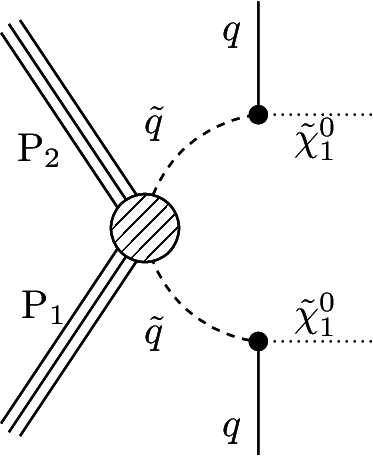
\includegraphics[width=.21\unitlength]{figures/pMSSMpaper/topologies/1_T2qq.png}}
         \put(0.11,-0.015){\makebox(0,0){\small (1) $\tilde{\rm q}\tilde{\rm q}(\tilde{\rm q} \hspace{-1mm}\rightarrow \hspace{-1mm}{\rm q}\tilde{\chi}_{1}^{0})$}}
        \end{picture}
}
\hspace{0mm}
  \makebox[.21\textwidth][c]{
        \setlength{\unitlength}{\linewidth}
        \begin{picture}(.21,.21)
         \put(0,0){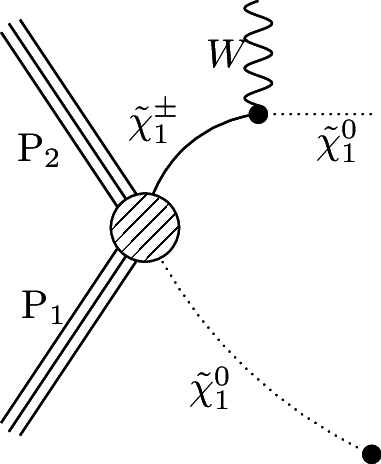
\includegraphics[width=.21\unitlength]{figures/pMSSMpaper/topologies/2_C1qq.png}}
         \put(0.11,-0.015){\makebox(0,0){\small (2) $\tilde{\chi}^{\pm}_{1}\tilde{\chi}^{0}(\tilde{\chi}^{\pm}_{1} \hspace{-1mm}\rightarrow \hspace{-1mm}{\rm W}^{\pm}\tilde{\chi}_{1}^{0})$}}
        \end{picture}
}
\hspace{0mm}
  \makebox[.21\textwidth][c]{
        \setlength{\unitlength}{\linewidth}
        \begin{picture}(.21,.21)
         \put(0,0){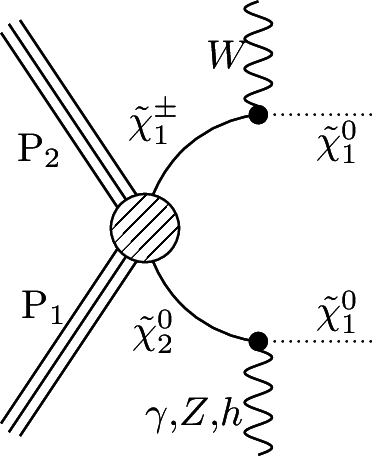
\includegraphics[width=.21\unitlength]{figures/pMSSMpaper/topologies/3_TChiWB.png}}
         \put(0.11,-0.015){\makebox(0,0){\small (3) $\tilde{\chi}^{\pm}_{1}\tilde{\chi}^{0}_{2}(\tilde{\chi} \hspace{-1mm}\rightarrow \hspace{-1mm}{\rm V/h}\tilde{\chi}_{1}^{0})$}}
        \end{picture}
}
\hspace{0mm}
  \makebox[.21\textwidth][c]{
        \setlength{\unitlength}{\linewidth}
        \begin{picture}(.21,.21)
         \put(0,0){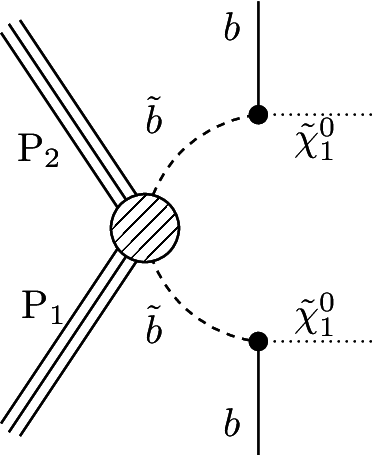
\includegraphics[width=.21\unitlength]{figures/pMSSMpaper/topologies/4_T2bb.png}}
         \put(0.11,-0.015){\makebox(0,0){\small (4) $\tilde{\rm b}\tilde{\rm b}(\tilde{\rm b} \hspace{-1mm}\rightarrow \hspace{-1mm}{\rm b}\tilde{\chi}_{1}^{0})$}}
        \end{picture}
}
\centering
\vspace{1.5cm}
\hspace{0mm}
  \makebox[.21\textwidth][c]{
        \setlength{\unitlength}{\linewidth}
        \begin{picture}(.21,.21)
         \put(0,0){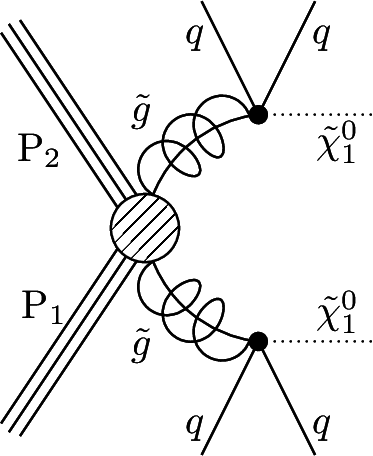
\includegraphics[width=.21\unitlength]{figures/pMSSMpaper/topologies/5_T1.png}}
         \put(0.11,-0.015){\makebox(0,0){\small (5) $\tilde{\rm g}\tilde{\rm g}(\tilde{\rm g} \hspace{-1mm}\rightarrow \hspace{-1mm}{\rm qq}\tilde{\chi}_{1}^{0})$}}
        \end{picture}
}
\hspace{0mm}
  \makebox[.21\textwidth][c]{
        \setlength{\unitlength}{\linewidth}
        \begin{picture}(.21,.21)
         \put(0,0){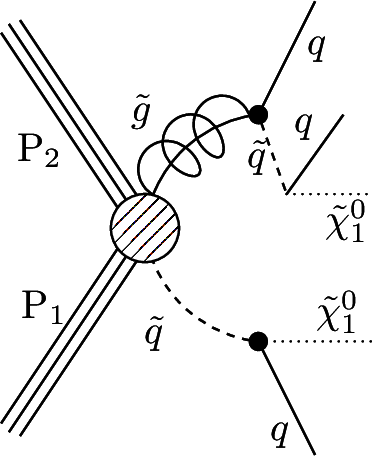
\includegraphics[width=.21\unitlength]{figures/pMSSMpaper/topologies/6_T3qqq.png}}
         \put(0.11,-0.015){\makebox(0,0){\small (6) $\tilde{\rm g}\tilde{\rm q}(\tilde{\rm g} \hspace{-1mm}\rightarrow \hspace{-1mm}\tilde{\rm q}{\rm q}\tilde{\chi}_{1}^{0})$}}
        \end{picture}
}
\hspace{0mm}
  \makebox[.21\textwidth][c]{
        \setlength{\unitlength}{\linewidth}
        \begin{picture}(.21,.21)
         \put(0,0){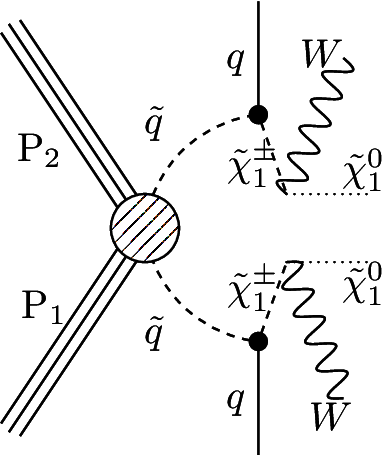
\includegraphics[width=.21\unitlength]{figures/pMSSMpaper/topologies/7_T4qqww.png}}
         \put(0.11,-0.015){\makebox(0,0){\small (7) $\tilde{\rm q}\tilde{\rm q}(\tilde{\rm q} \hspace{-1mm}\rightarrow \hspace{-1mm}{\rm q}\tilde{\chi}^{\pm}_{1})^{\text{*}}$}}
        \end{picture}
}
\hspace{0mm}
 \makebox[.21\textwidth][c]{
        \setlength{\unitlength}{\linewidth}
        \begin{picture}(.21,.21)
         \put(0,0){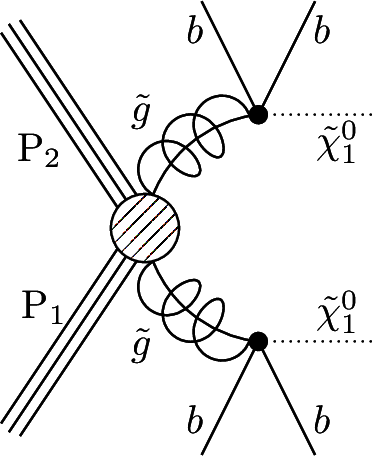
\includegraphics[width=.21\unitlength]{figures/pMSSMpaper/topologies/8_T1bb.png}}
         \put(0.11,-0.015){\makebox(0,0){\small (8) $\tilde{\rm g}\tilde{\rm g}(\tilde{\rm g} \hspace{-1mm}\rightarrow \hspace{-1mm}{\rm bb}\tilde{\chi}_{1}^{0})$}}
        \end{picture}
}
\centering
\vspace{1.5cm}
\hspace{0mm}
 \makebox[.21\textwidth][c]{
        \setlength{\unitlength}{\linewidth}
        \begin{picture}(.21,.21)
         \put(0,0){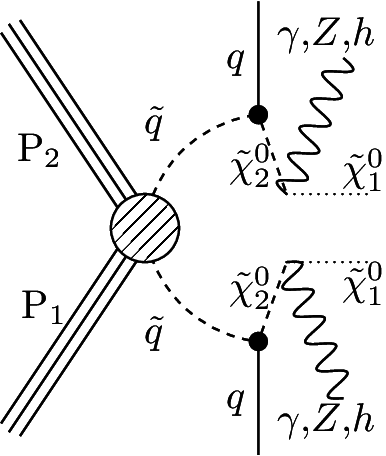
\includegraphics[width=.21\unitlength]{figures/pMSSMpaper/topologies/9_T4zz.png}}
         \put(0.11,-0.015){\makebox(0,0){\small (9) $\tilde{\rm q}\tilde{\rm q}(\tilde{\rm q} \hspace{-1mm}\rightarrow \hspace{-1mm}{\rm q}\tilde{\chi}^{0}_{2})^{\text{*}}$}}
        \end{picture}
}
\hspace{0mm}
 \makebox[.21\textwidth][c]{
        \setlength{\unitlength}{\linewidth}
        \begin{picture}(.21,.21)
         \put(0,0){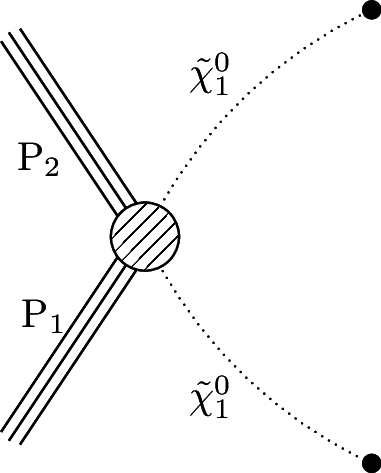
\includegraphics[width=.21\unitlength]{figures/pMSSMpaper/topologies/10_NN.png}}
         \put(0.11,-0.015){\makebox(0,0){\small (10) $\tilde{\chi}^{0}_{1}\tilde{\chi}^{0}_{1}$}}
        \end{picture}
}
\hspace{0mm}
 \makebox[.21\textwidth][c]{
        \setlength{\unitlength}{\linewidth}
        \begin{picture}(.21,.21)
         \put(0,0){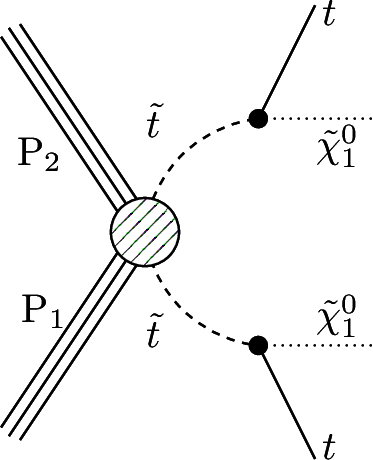
\includegraphics[width=.21\unitlength]{figures/pMSSMpaper/topologies/11_T2tt.png}}
         \put(0.11,-0.015){\makebox(0,0){\small (11) $\tilde{\rm t}\tilde{\rm t}(\tilde{\rm t} \hspace{-1mm}\rightarrow \hspace{-1mm}{\rm t}\tilde{\chi}_{1}^{0})$}}
        \end{picture}
}
\hspace{0mm}
\makebox[.21\textwidth][c]{
        \setlength{\unitlength}{\linewidth}
        \begin{picture}(.21,.21)
         \put(0,0){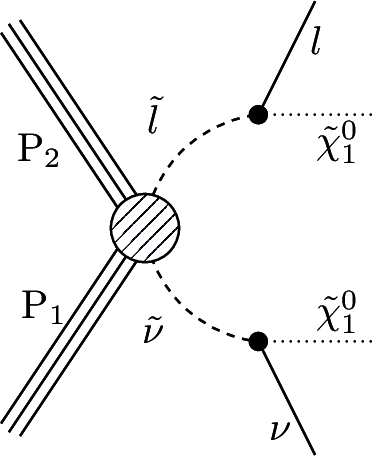
\includegraphics[width=.21\unitlength]{figures/pMSSMpaper/topologies/12_LSnu.png}}
         \put(0.11,-0.015){\makebox(0,0){\small (12) $\tilde{\rm l}^{\pm}\tilde{\nu}(\tilde{\rm l} \hspace{-1mm}\rightarrow
\hspace{-1mm}{\rm l}\tilde{\chi}_{1}^{0})$}}
        \end{picture}
}
\vspace{6 mm}
\caption{The twelve most common principal processes in the pMSSM, listed in order 
of their frequency before the constraints of the CMS searches. Both on-shell and off-shell states are included.
 Indices of particle charge, flavor, and chirality are ignored in the construction, with the exception of the flavor of the third-generation squarks and quarks. Asterisks in the labels indicate where process names involving long decay chains have been abbreviated.}
\label{fig:diagrams1}
\end{figure}


The distribution of principal processes for excluded and nonexcluded
points is given in Fig.~\ref{fig:TopoHisto} (a).  It is seen that processes
involving direct gluino production (5 and 8) are excluded with
a much higher
frequency than they survive, and those with EW
gaugino production (2, 3, and 10) survive with a higher frequency than they are
excluded. Processes with first-generation squark production (1 and 7) survive
and are excluded at similar rates, and processes with
slepton production (12) have exceptionally high survival rates. 
These trends are likely attributable to the difference in the
production cross section between colored and noncolored particles for
a given SUSY mass scale. 
The overflow bin (other), which contains many principal
processes, including modes of colored and noncolored particle
production, indicates a survival rate approximately equal to the
exclusion rate.  
The dominance is defined for each model point
as the ratio of the cross section of the principal process to the total SUSY
production cross section at 8~\TeV, 
 \begin{equation}
  {\rm dominance} \equiv \sigma^{8~\TeV~}_{\rm principal}/\sigma^{8~\TeV~}_{\rm tot},
  \label{eq:dominance}
\end{equation}
and is shown in Fig.~\ref{fig:TopoHisto} (b). Most values of the dominance are in the
range 0.05\textendash0.60. The excluded and nonexcluded values for the
dominance are seen to agree within the RMS of the distributions, indicating that the
presence of multiple event types within a single model
hypothesis does not
significantly impact our ability to exclude such a model point.
\begin{figure}[tb!]
  \centering
  \makebox[.647\textwidth][c]{
        \setlength{\unitlength}{\linewidth}
        \begin{picture}(.647,.647)
         \put(0,0){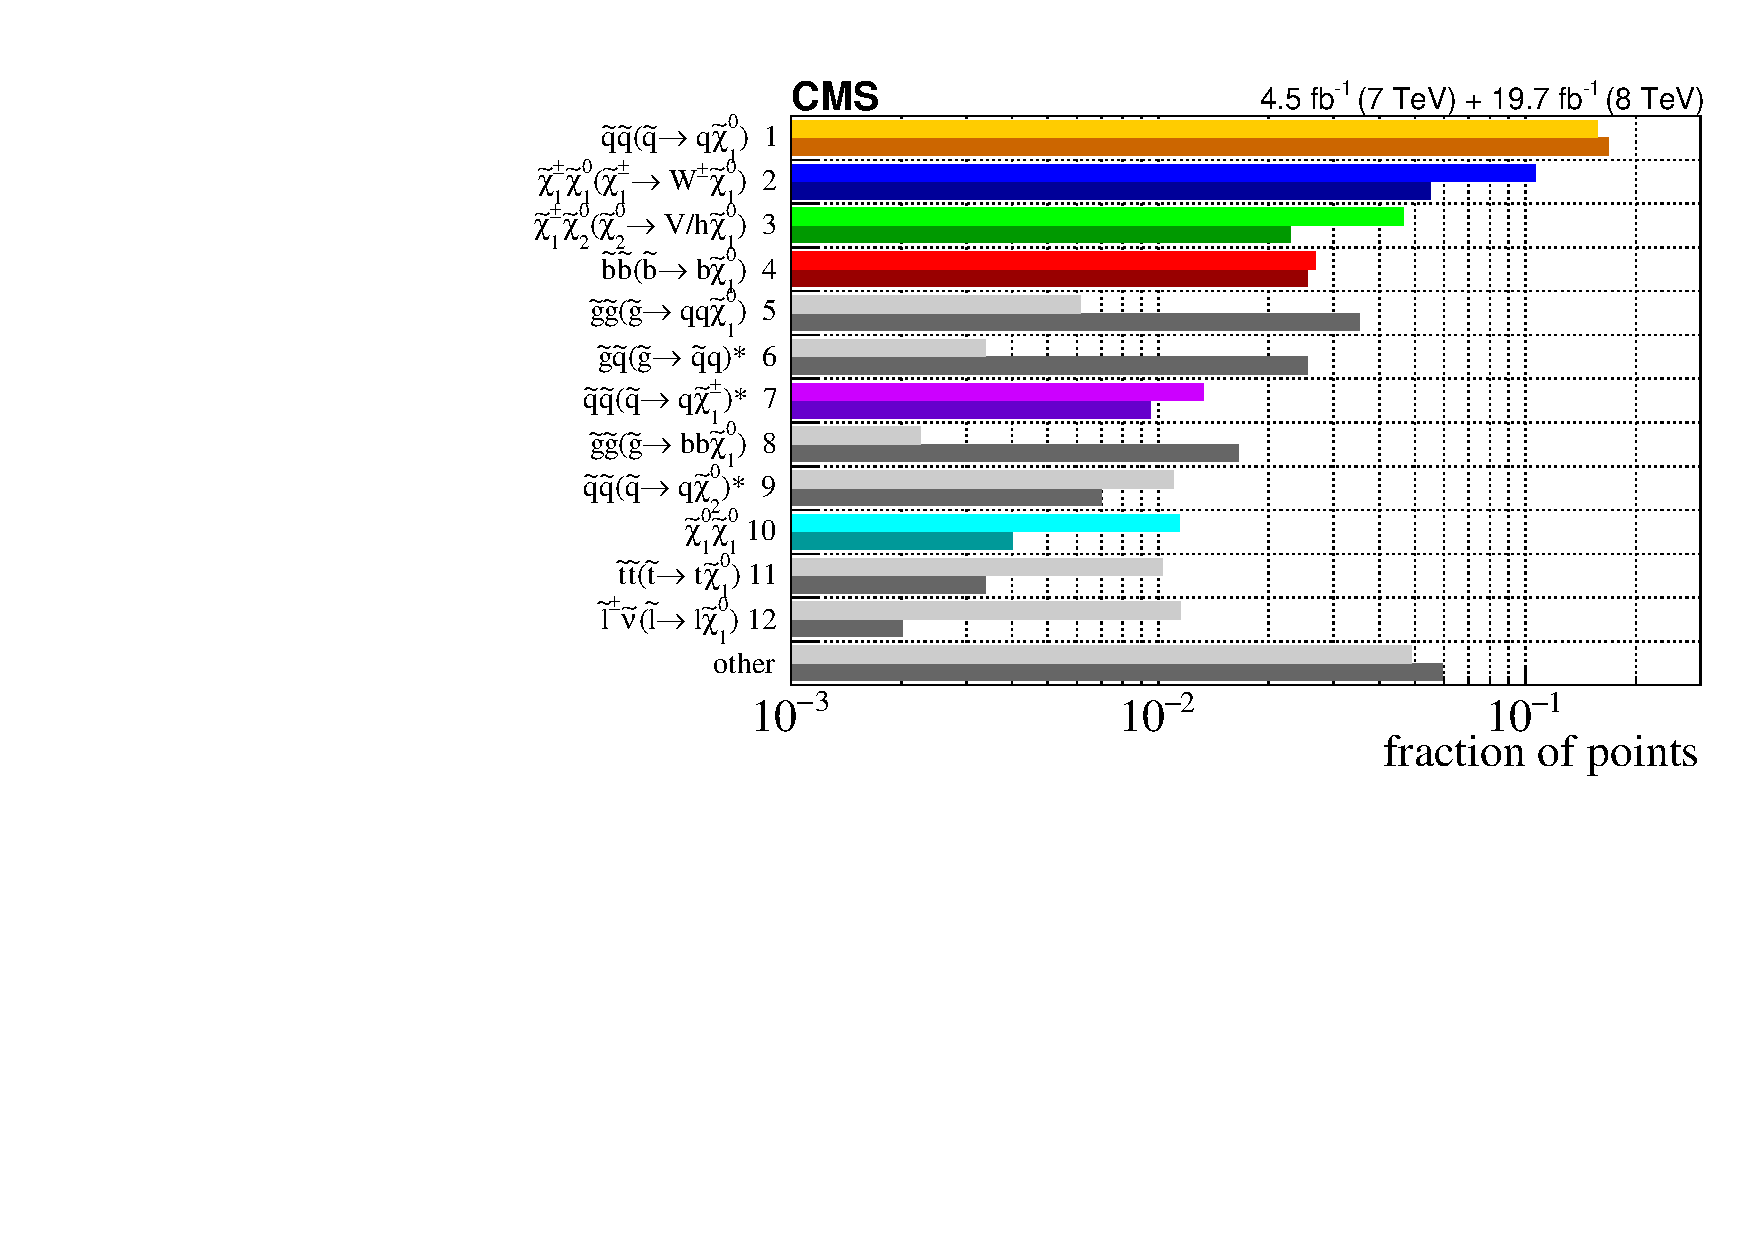
\includegraphics[width=.647\unitlength]{figures/pMSSMpaper/topologies/PrincipalProcesses.pdf}\label{fig:TopoHistoA}}
         \put(0.375,-.0){\scriptsize (a)}
        \end{picture}
}
  \makebox[.344\textwidth][c]{
        \setlength{\unitlength}{\linewidth}
        \begin{picture}(.344,.344)
         \put(0,0){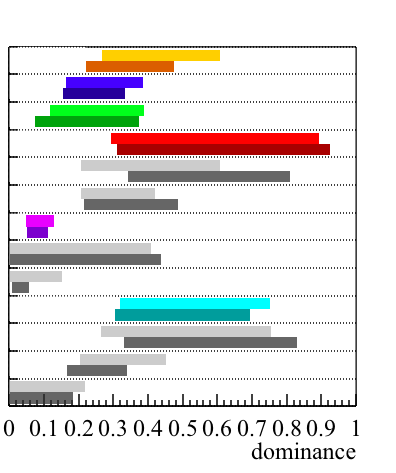
\includegraphics[width=.344\unitlength]{figures/pMSSMpaper/topologies/Dominance.png}\label{fig:TopoHistoB}}
         \put(0.145,-.0){\scriptsize (b)}
        \end{picture}
        }
    \caption{(a) shows the fraction of excluded
  (dark) and nonexcluded (light) points out of all considered points,
  by principal process. Color is assigned to the processes that are most common after the constraints of the CMS searches, which are selected for further study. The dominance
  of principal processes, as defined in Eq.~\ref{eq:dominance}, is given in (b) where the bands show the
  RMS range of the dominance. }
    \label{fig:TopoHisto}
\end{figure}
\FloatBarrier

Dedicated searches exist that correspond to some of the most frequent principal processes, indicating areas where the SMS approach is likely well optimized. For example, points with principal processes 1, $\tilde{\rm q}\tilde{\rm q}(\tilde{\rm q} \hspace{-1mm}\rightarrow \hspace{-1mm}{\rm q}\tilde{\chi}_{1}^{0})$, and 4, $\tilde{\rm b}\tilde{\rm b}(\tilde{\rm b} \hspace{-1mm}\rightarrow \hspace{-1mm}{\rm b}\tilde{\chi}_{1}^{0})$, enjoy searches that target these processes explicitly.   A few principal processes have not been explicitly targeted by the host of CMS SUSY searches, including processes 2, $\tilde{\chi}^{\pm}_{1}\tilde{\chi}^{0}(\tilde{\chi}^{\pm}_{1} \hspace{-1mm}\rightarrow \hspace{-1mm}{\rm W}^{\pm}\tilde{\chi}_{1}^{0})$, and 3, $\tilde{\chi}^{\pm}_{1}\tilde{\chi}^{0}_{2}(\tilde{\chi} \hspace{-1mm}\rightarrow \hspace{-1mm}{\rm V/h}\tilde{\chi}_{1}^{0})$, the asymmetric EW gaugino production modes. New searches that target these or the other overlooked processes may serve to broaden the overall sensitivity to the pMSSM.


\subsection{Characterization of signal events}
Next, the nonexcluded model space is characterized by the predicted
final states in order to shed light on what signatures may serve to target the nonexcluded points in Run 2.  A loose set of baseline physics objects and event 
variables are defined at the generator level, as follows:
\begin{itemize}
\item Leptons: electrons, muons, or taus having a transverse momentum $p_{\rm T}$ greater than 5 GeV and an isolation less than 0.2. Here, isolation  =
$[(\Sigma_{i}{p_{\rm T}}_i) - p_{\rm T}]/\Sigma_{i}{p_{\rm T}}_i$,
where the sums run over all detector-visible particles $i$ within a
$\Delta$R cone of 0.5 around the object, with $\Delta$R = $\sqrt{(\Delta\eta)^2+(\Delta\phi)^2}$;
%\item Photons: photons having a $p_{\rm T}$ greater than 5\GeV and an isolation less than 0.2, with the same definition of isolation as for leptons;
\item Jets: particles clustered with the anti-kT jet algorithm \cite{Cacciari:2008gp} with distance parameter 0.5. The jets are required to have a $p_{\rm T}$ greater than 20 GeV;
\item b-jets: jets matched to a b hadron within a $\Delta$R of 0.5;
\item \MET{}: the missing transverse energy, calculated as the magnitude
  of the vector sum of the transverse momenta of
 visible particles with $p_{\rm T} >$ 5 GeV; 
\item \HT{}: the scalar sum of the $p_{\rm T}$ of the jets with
  a $p_{\rm T}>$ 50 GeV.
%\item MHT: the scalar sum of the transverse momenta of the jets with a $p_{\rm T}>$ 30\GeV
%\item $\Delta \phi($MHT$, jet_{1})$: The average azimuthal separation between the leading jet and the 
%missing \HT{} for events with at least three 50\GeV jets and no isolated leptons or photons.
\end{itemize}

A parallel coordinates visualization technique is used that enables the
display of multiple dimensions (as introduced in Chapter \ref{chap:SM}). Figure~\ref{fig:parcor},
shows nonexcluded points corresponding to the six selected
principal processes (those denoted by color in Fig.~\ref{fig:parcor}).
Vertical axes are chosen to represent meaningful properties of the model
points, and each model point is represented as a curved line traversing the plot from left to right, intersecting each axis at the parameter value taken by the model point. The curvature of the lines is added to help distinguish between similar pMSSM points, but the trajectories of the lines between the axes do not carry physical information. A number of distinct scenarios are seen to have survived the CMS
analyses.  A minimum threshold of 20 fb has been applied to the 8~\TeV~ signal
cross sections to limit the scope to those
points that could potentially still be probed with the Run 1 data set
using an expanded set of analyses and techniques.


\begin{figure}[tb!]
  \centering
         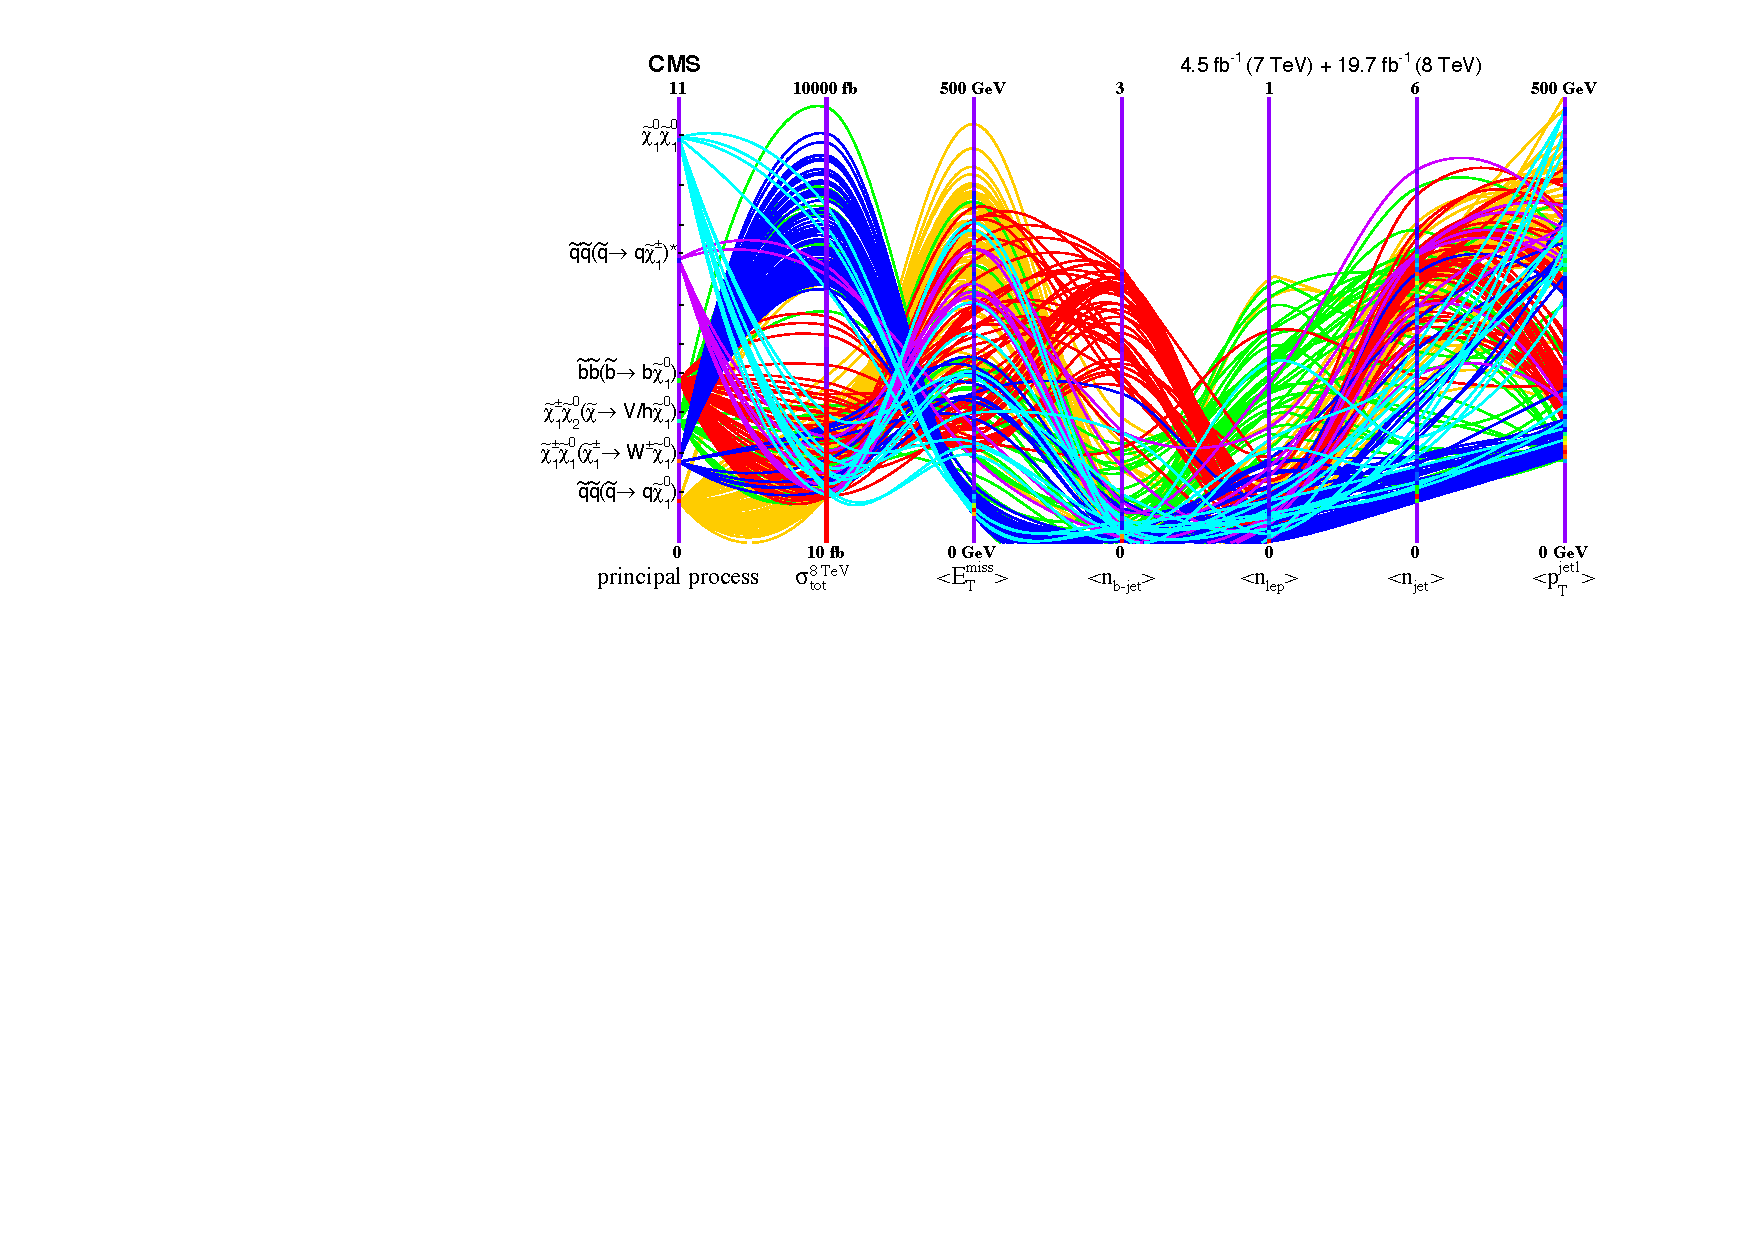
\includegraphics[width=1.0\linewidth]{figures/pMSSMpaper/parallel_coordinates/ParCorTopos.pdf}
    \caption{A parallel coordinates plot showing several hundred
      selected nonexcluded model points for the six most common
      principal processes, with seven key properties.
      From the left, the selected properties are: the principal
      process, the 8~\TeV~ signal production cross section (in
      log$_{\text{10}}$ scale), the average value of the \MET{}, the average number of
      b-jets, leptons, and jets, and finally, the average $p_{T}$
      momentum of the leading jet. Color is assigned based on the
      principal process. Orange codes for process 1, blue for
      process 2, green for 3, red for 4, violet for 7, and 
      cyan for 10.  Lines
      arching toward higher vertical positions typically indicate more
      ``discoverable'' scenarios. }
    \label{fig:parcor}
\end{figure}


The nonexcluded points associated with principal processes 1, $\tilde{\rm q}\tilde{\rm q}(\tilde{\rm q} \hspace{-1mm}\rightarrow \hspace{-1mm}{\rm q}\tilde{\chi}_{1}^{0})$, and 4, $\tilde{\rm b}\tilde{\rm b}(\tilde{\rm b} \hspace{-1mm}\rightarrow \hspace{-1mm}{\rm b}\tilde{\chi}_{1}^{0})$, are seen to give rise to large average \MET{}, jet multiplicities between 2 and 4, and moderate to low cross sections due the the large masses of the squarks. Given the
higher cross sections in Run 2, these high \MET{} scenarios will become increasingly more accessible.

Model points with principal processes 2, $\tilde{\chi}^{\pm}_{1}\tilde{\chi}^{0}(\tilde{\chi}^{\pm}_{1} \hspace{-1mm}\rightarrow \hspace{-1mm}{\rm W}^{\pm}\tilde{\chi}_{1}^{0})$, and 3, $\tilde{\chi}^{\pm}_{1}\tilde{\chi}^{0}_{2}(\tilde{\chi} \hspace{-1mm}\rightarrow \hspace{-1mm}{\rm V/h}\tilde{\chi}_{1}^{0})$, typically predict large cross sections, in the range 100 fb pb, 
but a limited number of physical observables, primarily due to compression in the mass spectrum between the LSP and the other EW gauginos. These points peak low in the average multiplicity of jets, leptons, and in average \MET{}. They could potentially be probed with searches that involve events with initial state radiation and soft boson decay products that are aligned with the \MET{}.

Points with principal processes 3, $\tilde{\chi}^{\pm}_{1}\tilde{\chi}^{0}_{2}(\tilde{\chi} \hspace{-1mm}\rightarrow \hspace{-1mm}{\rm V/h}\tilde{\chi}_{1}^{0})$, and 10, $\tilde{\chi}^{0}_{1}\tilde{\chi}^{0}_{1}$, tend to follow the trend profiled
by process 2, $\tilde{\chi}^{\pm}_{1}\tilde{\chi}^{0}(\tilde{\chi}^{\pm}_{1} \hspace{-1mm}\rightarrow \hspace{-1mm}{\rm W}^{\pm}\tilde{\chi}_{1}^{0})$, differing primarily in the lepton multiplicity and, in the case of at least one lepton, in the average $\pt$ of the highest-$\pt$ lepton (leading lepton). The close resemblance of
processes 10 and 2  is mostly due to the fact that the mass
difference between the $\tilde{\chi}_{1}^\pm$ and
$\tilde{\chi}_1^0$ is frequently very small (less than 1 GeV), causing the ensuing off-shell W 
boson of process 2 to produce undetectably soft particles.

Points with principal processes 5, $\tilde{\rm g}\tilde{\rm g}(\tilde{\rm g} \hspace{-1mm}\rightarrow \hspace{-1mm}{\rm qq}\tilde{\chi}_{1}^{0})$, and 6, $\tilde{\rm g}\tilde{\rm q}(\tilde{\rm g} \hspace{-1mm}\rightarrow \hspace{-1mm}\tilde{\rm q}{\rm q}\tilde{\chi}_{1}^{0})$, the most frequent modes
involving gluinos, are not highlighted in Fig.~\ref{fig:parcor}, since their frequency among nonexcluded points is relatively small. Several of the nonexcluded models with very light gluino masses (less than 700 GeV) correspond to principal process 6, with mass differences between the $\tilde{\text{g}}$ and LSP that range around 100~\GeV. Sensitivity to these model points may be possible by considering final states with three or fewer jets and \MET{} thresholds that are lower than typically applied.

Points with principal process 7, $\tilde{\rm q}\tilde{\rm q}(\tilde{\rm q} \hspace{-1mm}\rightarrow \hspace{-1mm}{\rm q}\tilde{\chi}^{\pm}_{1})^{\text{*}}$, do not display distinct trends in the
properties selected, which is partly due to these points having a
low dominance of around 0.1. Such model points have a diverse set of
secondary processes, which are not directly examined here.

A general observation about the model points in Fig.~\ref{fig:parcor}
is the significant anticorrelation of observables, which
manifests as the criss-crossing of lines between the axes. For example,
model points with very high average \MET{} tend to have very low cross sections,
and vice versa. This is a consequence of the fact that, having observed no significant excess of events in data,
the surviving model points are those with very few experimentally accessible 
observables, or they would have been excluded.

\subsubsection{Signal fiducial cross sections}
With over 50\%
of all nonexcluded points corresponding to cross sections of
greater than 10 fb, it is critical to further examine why these points were not accessed in Run 1.  
To attempt to gain an
understanding, the signal is further characterized by evaluating fiducial cross sections corresponding to a
range of final-state observables. The fiducial cross section
$\sigma_{\text{f}}$ of a final-state is defined for each model point as 
 \begin{equation}
   \sigma_{\text{f}} = \sigma_{\text{tot}}^{\text{8 TeV}}A,
\end{equation}
where {\it A} is the acceptance times signal efficiency
computed as the fraction of simulated signal events
passing a set of event-level criteria. 
A set of final-state observables are examined that loosely correspond to trigger thresholds or
signal regions of the examined searches. Figures
\ref{fig:parcorMET}-\ref{fig:parcorBJet1} show the impact of adjusting
various thresholds on the fiducial cross sections of nonexcluded points.
\begin{figure}[tb!]
  \centering
         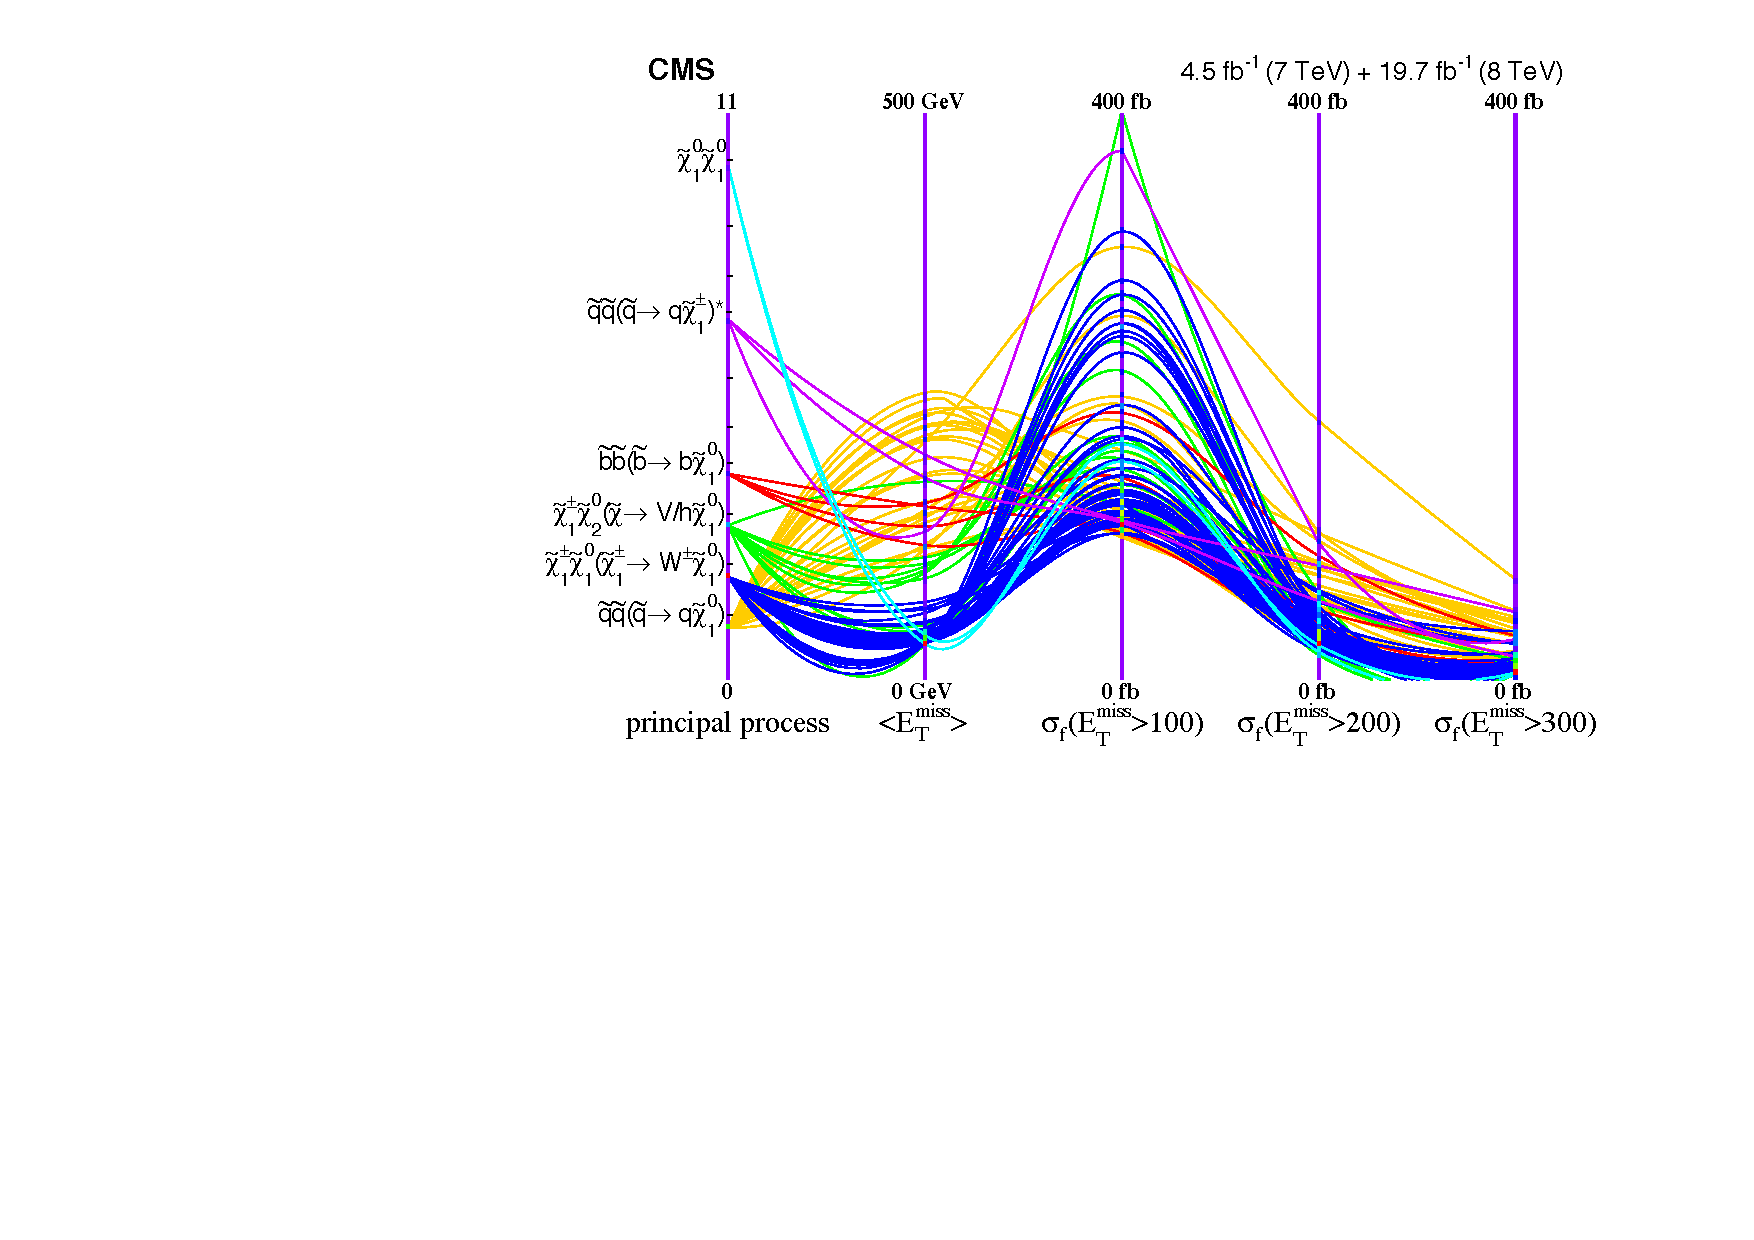
\includegraphics[width=0.9\textwidth]{figures/pMSSMpaper/parallel_coordinates/ParCorToposMET.pdf}
    \caption{A parallel coordinates plot of the nonexcluded pMSSM points
      with the axes set as the principal process, the average \MET{} (in GeV), and the 
    fiducial cross section (in linear scale) for various thresholds on the
    \MET{}. All nonexcluded points corresponding to processes 1, 2, 3,
    4, 7, and 10 that have a fiducial cross section greater than 100 fb are shown. Color is
    assigned to values of the principal process in the same manner as
    in Fig.~\ref{fig:parcor}.}
    \label{fig:parcorMET}
\end{figure}
\begin{figure}[tb!]
  \centering
         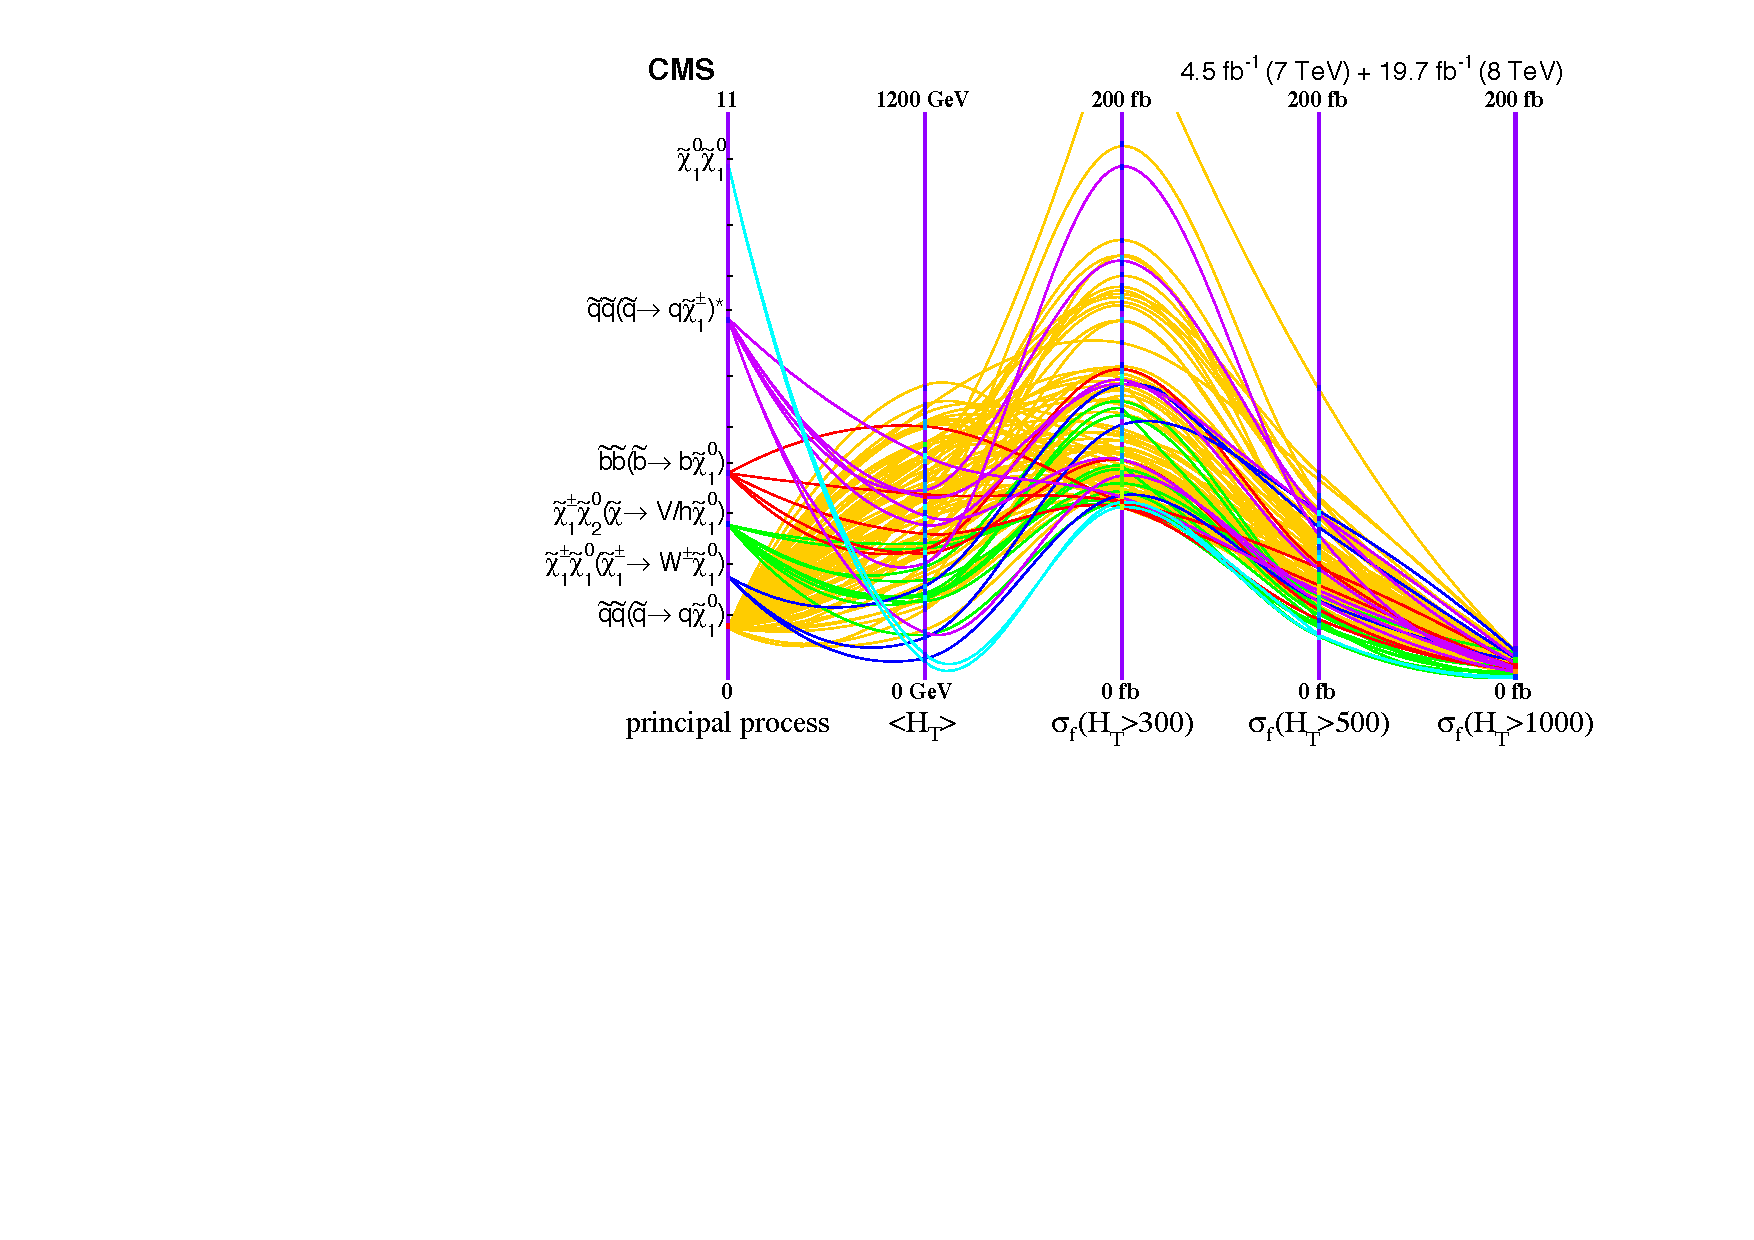
\includegraphics[width=0.9\textwidth]{figures/pMSSMpaper/parallel_coordinates/ParCorToposHT.pdf}
    \caption{A parallel coordinates plot of the nonexcluded pMSSM
      points with the axes set as the principal process, the average
      \HT{} (in GeV), and the 
    fiducial cross section (in linear scale) for various thresholds on the
    \HT{}. All nonexcluded points corresponding to processes 1, 2, 3,
    4, 7, and 10 that have a fiducial cross section greater than
    60 fb
    are shown. Color is assigned to
    values of the principal process in the same manner as in
    Fig.~\ref{fig:parcor}. }
    \label{fig:parcorHT}
\end{figure}
\begin{figure}[tb!]
  \centering
         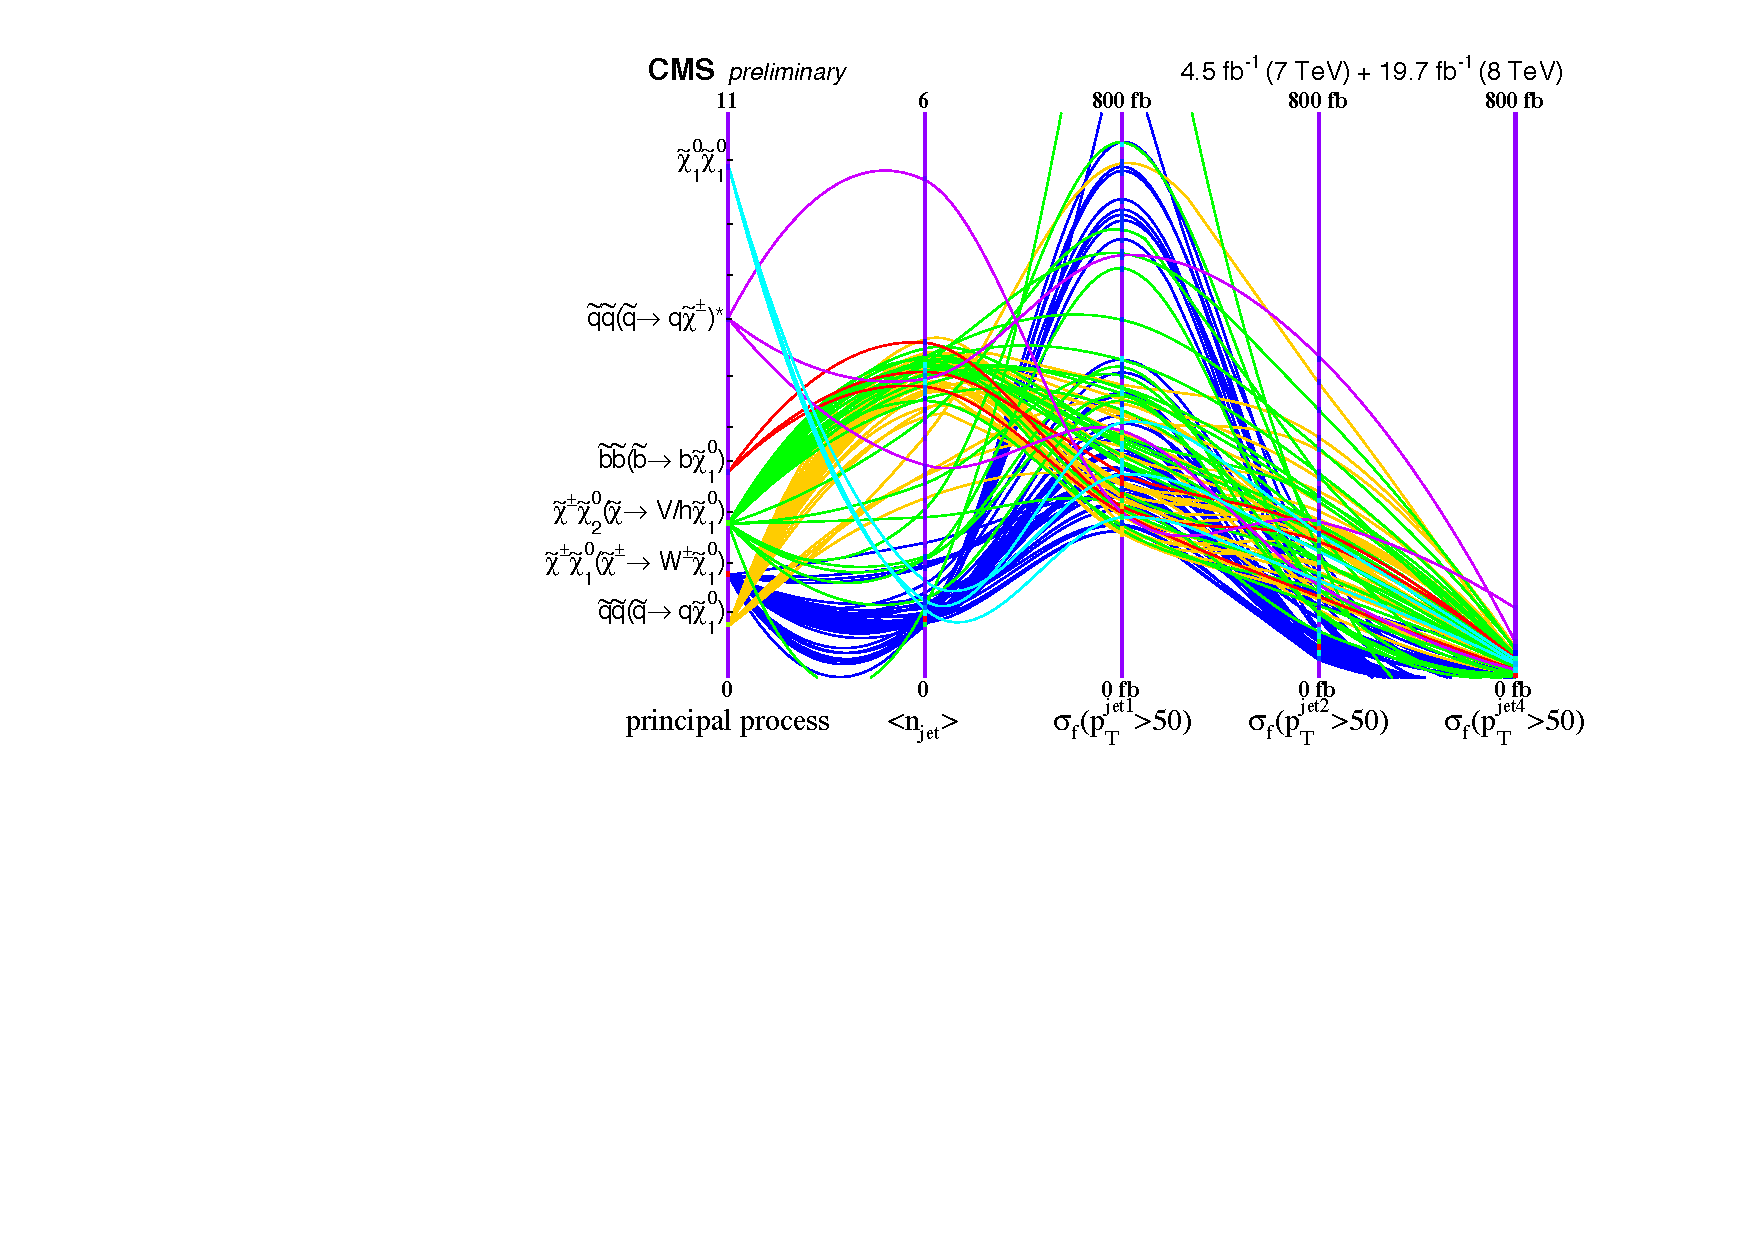
\includegraphics[width=0.9\textwidth]{figures/pMSSMpaper/parallel_coordinates/ParCorToposJets.pdf}
    \caption{A parallel coordinates plot of the nonexcluded pMSSM
      points with the axes set as the principal process and the 
    fiducial cross section (in linear scale) for various thresholds on the
    multiplicity of jets. All nonexcluded points corresponding to processes 1, 2, 3,
    4, 7, and 10 that have a fiducial cross section greater than 200 fb are shown. Color is
    assigned to values of the principal process in the same manner as
    in Fig.~\ref{fig:parcor}. } 
    \label{fig:parcorNJets}
\end{figure}
\begin{figure}[tb!]
  \centering
   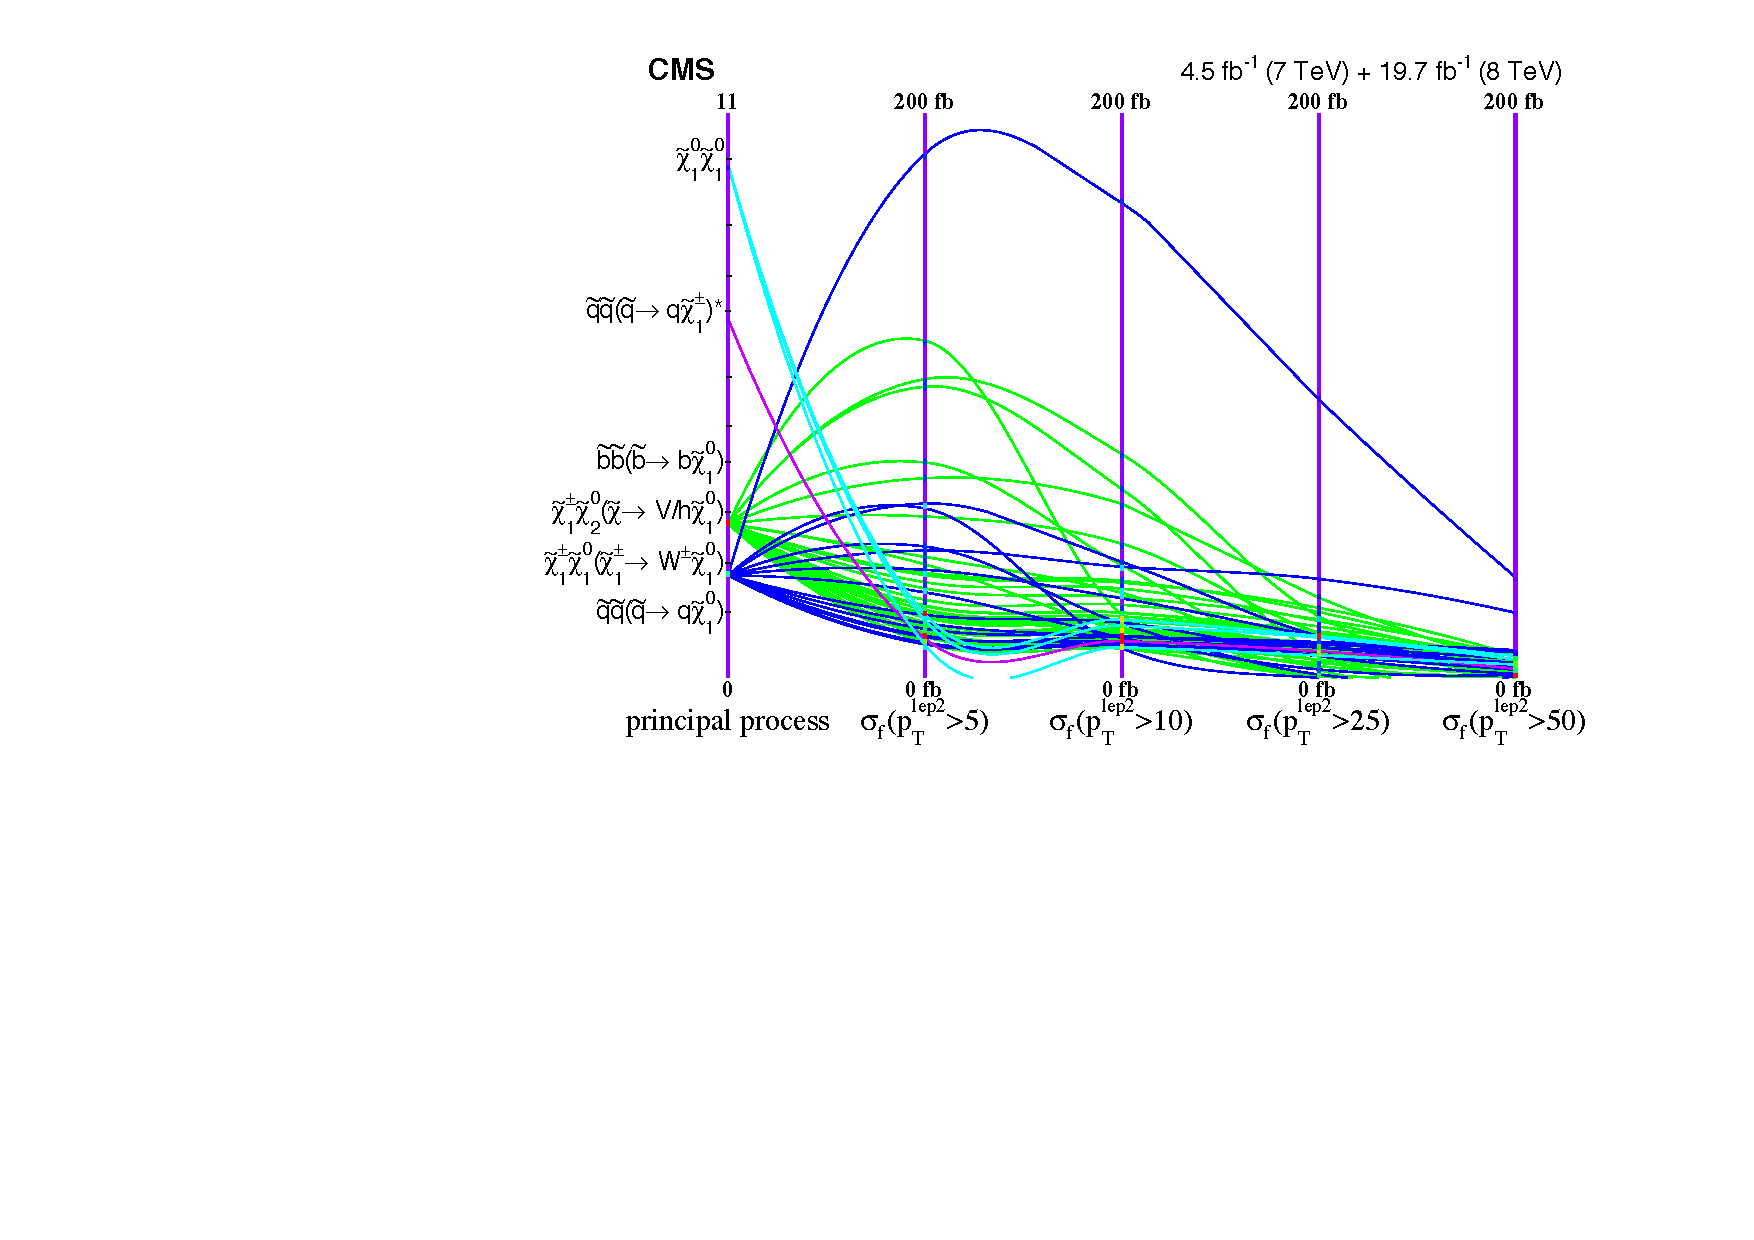
\includegraphics[width=0.9\textwidth]{figures/pMSSMpaper/parallel_coordinates/ParCorToposLep2.pdf}
    \caption{A parallel coordinates plot of the nonexcluded pMSSM
      points with the axes set as the principal process and the 
    fiducial cross section (in linear scale) for various thresholds on the
    sub-leading lepton $p_{\rm T}$ (in GeV). All nonexcluded points corresponding to processes 1, 2, 3,
    4, 7, and 10 that have a fiducial cross section greater than 30 fb are shown. Color is
    assigned to values of the principal process in the same manner as
    in Fig.~\ref{fig:parcor}. } 
    \label{fig:parcorLEP2}
\end{figure}
\begin{figure}[tb!]
  \centering
   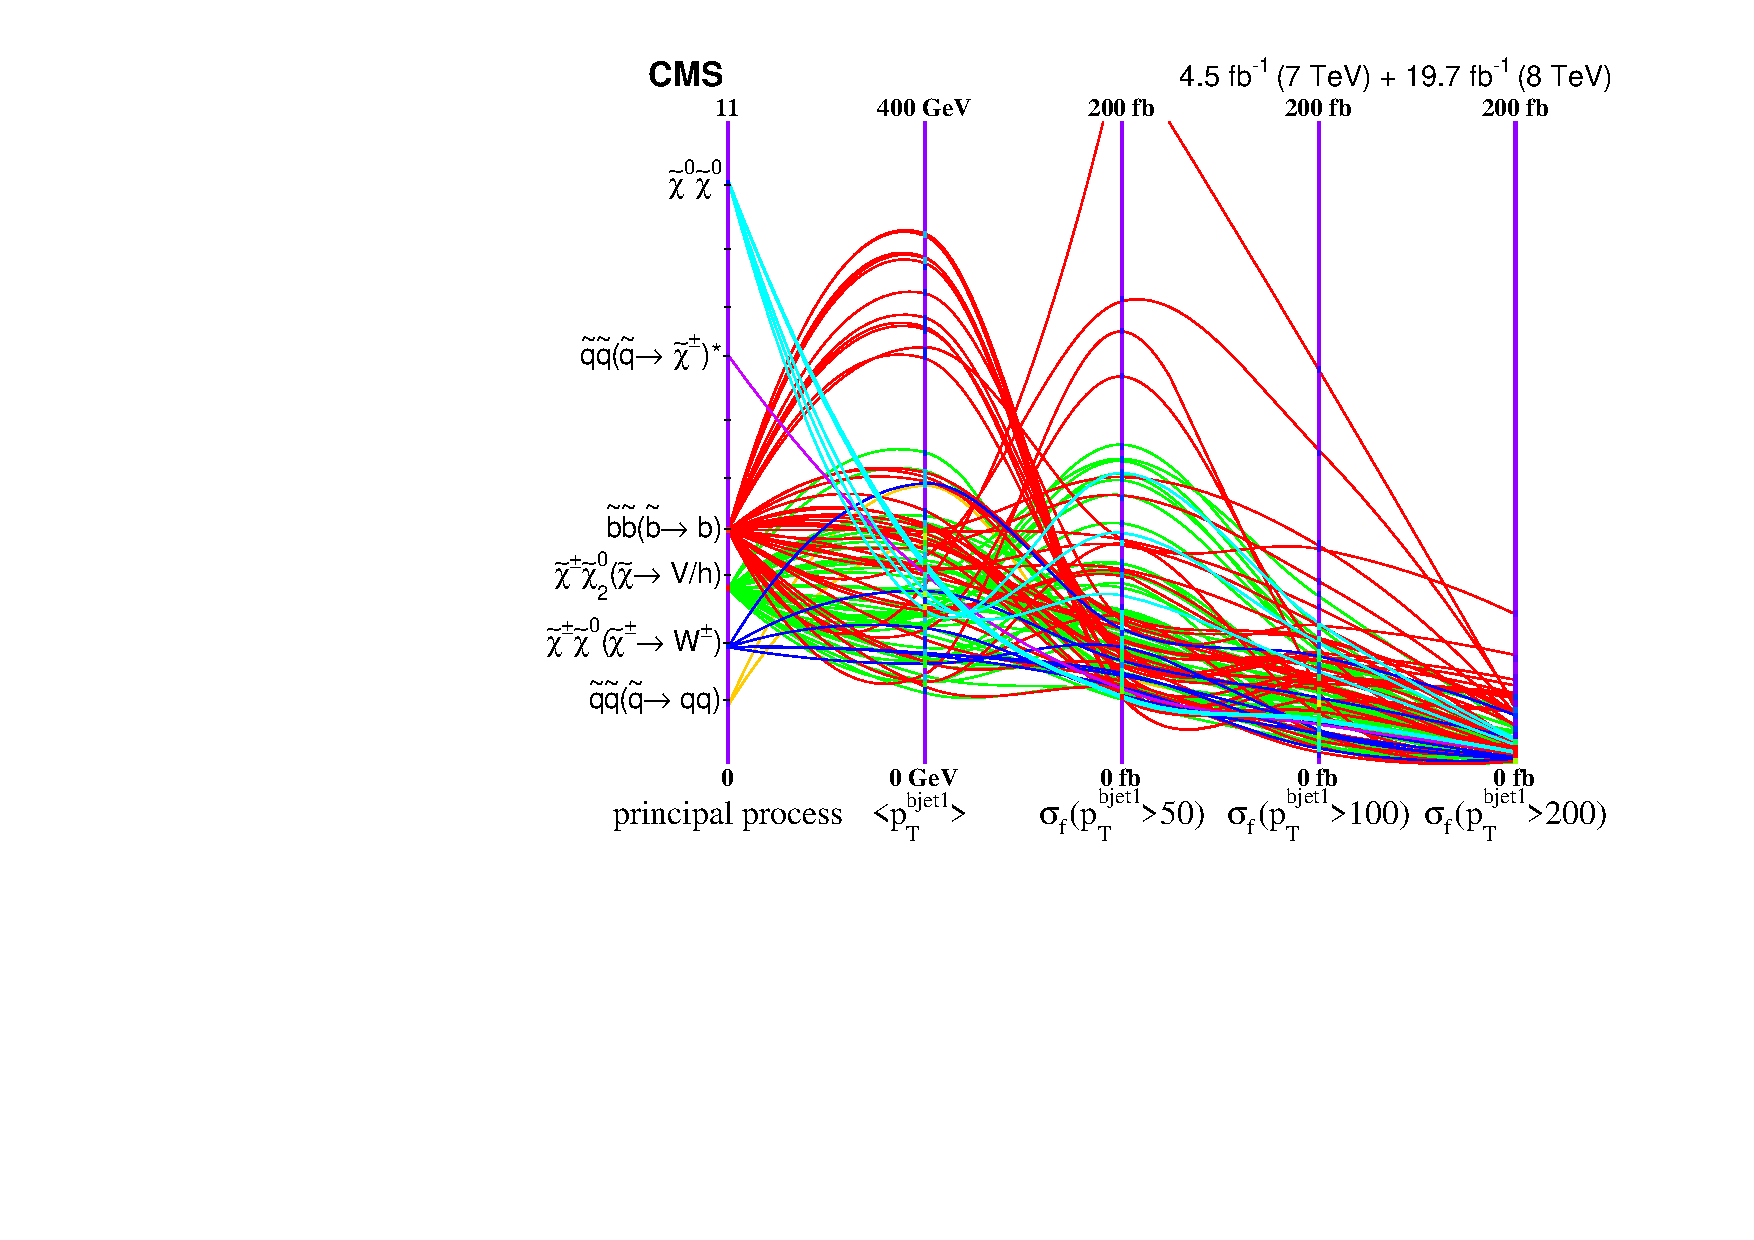
\includegraphics[width=0.9\textwidth]{figures/pMSSMpaper/parallel_coordinates/ParCorToposBjet1.pdf}
    \caption{A parallel coordinates plot of the nonexcluded pMSSM
      points with the axes set as the principal process and the 
    fiducial cross section (in linear scale) for various thresholds on the
    leading b-tagged jet $p_{\rm T}$ (in GeV). All nonexcluded points corresponding to processes 1, 2, 3,
    4, 7, and 10 that have a fiducial cross section greater than 20 fb are shown. Color is
    assigned to values of the principal process in the same manner as
    in Fig.~\ref{fig:parcor}. } 
    \label{fig:parcorBJet1}
\end{figure}

Some principal processes can be associated with large fiducial
cross sections, depending on the final state considered. For example, points with mostly
first-generation squark production give rise to large
fiducial cross sections for events with high \HT{}, resulting in Fig.
\ref{fig:parcorHT} showing mostly orange-colored points; and points with production involving EW gauginos give rise to substantial
fiducial cross sections for events with a high multiplicity of soft leptons, which
explains the unaccompanied blue and green lines in Fig.~\ref{fig:parcorLEP2}.  Somewhat striking is the behavior of the \MET{} fiducial cross section
(Fig.~\ref{fig:parcorMET}), which can increase rapidly (by up to a
factor of ten) as the threshold
is relaxed from 200 to 100 GeV. It is apparent that many of the
nonexcluded regions are not accessible with thresholds of 200 GeV, 
a common criterion applied offline to achieve full efficiency
with the triggers. The fiducial cross section decreases noticeably as the
threshold is further increased from 200 to 300 GeV. Similar behavior is seen for the \HT{} fiducial cross section
(Fig.~\ref{fig:parcorHT}). Fiducial cross
sections are quite large for these final states when a
threshold of 300 GeV is applied, but fall off substantially for higher
thresholds. 

Of course, a loosening of the object thresholds would increase the background yield as well as signal yield. Therefore, a thorough survey of analysis techniques and specific backgrounds will be necessary 
to select optimal values for kinematic thresholds and other analysis techniques to probe the most difficult points. However, the lesson that nonexcluded pMSSM models have large cross sections in background-rich kinematic regions is an open invitation for the development of new techniques that improve signal to background discrimination and background modeling. If the MSSM is realized in one of these difficult regions, the hunt for SUSY will force us to either abandon the LHC, or become more creative. 

\FloatBarrier
\subsubsection{A note on low-mass gluinos}
Model points with gluino masses as low as 600 GeV survive CMS analyses, but these scenarios do not correspond to the top 12 processes listed in Fig. \ref{fig:diagrams1}. Such model points are characterized primarily by the processes shown in Fig. \ref{fig:diagrams2}. The intermediate EWkinos in the gluino decay chains serve to lower the $\pt$ of jets, and therefore $\Ht$, in signal events. Furthermore, the scenarios tend to have mass splittings between the gluino and LSP of less than a few hundred GeV, which leaves little kinetic energy available for the intermediate decay bosons, which are typically off shell. These features lead to a lowered signal efficiency in searches that require high jet multiplicity and large $\Ht$. These scenarios may be probed by searches with relatively low or moderate thresholds on the $\Ht$ and $\mht$, and by requiring initial state radiation to boost the SUSY particles into one single hemisphere. Then, requiring potentially soft decay products of the gluinos to be traveling in the direction of the $\met$ may serve to separating signal events from the number of QCD and $\zinv$ background events. In the case of Fig. \ref{fig:diagrams2} (b), requiring an identified track that disappears in the tracker,  a possible signature of the long-lived chargino, may greatly increase the sensitivity of searches in the case that the LSP and $\tilde{\chi}^{\pm}$ are sufficiently degenerate in mass.
\begin{figure}[tb!]
\centering
%\renewcommand*\thesubfigure{\arabic{subfigure}}
\hspace{0mm}
  \makebox[.25\textwidth][c]{
        \setlength{\unitlength}{\linewidth}
        \begin{picture}(.21,.21)
         \put(0,0){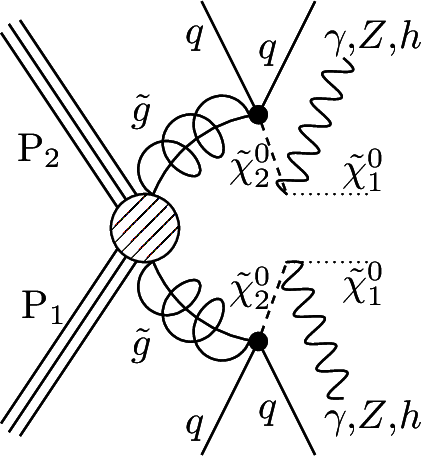
\includegraphics[width=.21\unitlength]{figures/pMSSMpaper/topologies/18_TLowGlue1.png}}
         \put(0.11,-0.015){\makebox(0,0){\small (18) $\tilde{\rm g}\tilde{\rm g}(\tilde{\rm g} \hspace{-1mm}\rightarrow \hspace{-1mm}{\rm 2qV}^0{\rm /h,\,}\tilde{\chi}_{1}^{0})$}}
        \end{picture}
}
\hspace{0mm}
  \makebox[.25\textwidth][c]{
        \setlength{\unitlength}{\linewidth}
        \begin{picture}(.21,.21)
         \put(0,0){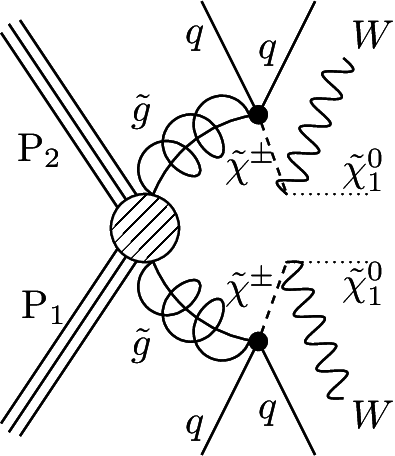
\includegraphics[width=.21\unitlength]{figures/pMSSMpaper/topologies/34_TLowGlue2.png}}
         \put(0.11,-0.015){\makebox(0,0){\small (34) $\tilde{\rm g}\tilde{\rm g}(\tilde{\rm g} \hspace{-1mm}\rightarrow \hspace{-1mm}{\rm 2qW}^\pm{\rm /h,\,}\tilde{\chi}_{1}^{0})$}}
        \end{picture}
}
\vspace{6 mm}
\caption{The 18$^{\rm th}$ and 34$^{\rm th}$ most frequent principal process in the pMSSM. }
\label{fig:diagrams2}
\end{figure}
